\chapter{Adversarial Markov Games: On Adaptive Offensive and Defensive Strategies}\label{ch:markovgames}
\label{ch:markovgames}

\section*{Preamble}

Despite considerable efforts on making them robust, real-world ML-based systems remain vulnerable to decision based attacks, as definitive proofs of their operational robustness have so far proven intractable for any but the simplest models.
The canonical approach in robustness evaluation calls for adaptive attacks, which draw parallels to the Kerckhoffs' principle in cryptography, namely that the security of a model should not rely on the secrecy about the model or its defenses. 
Adaptive attacks are therefore attacks that have complete knowledge of any defense and access to all the available tools to bypass them.
In this chapter, we take the notion of being adaptive a step further, by introducing a more expansive notion of it, while showing how attacks and also defenses can benefit by being adaptive \emph{and} by learning from each other through interaction.

We introduce a novel framework for adaptively optimizing black-box attacks and defenses against each other through the competitive game they form.
We initiate our investigation by focusing on adapting attacks: to reliably measure robustness it is paramount to evaluate against realistic and worst-case attacks.
It is not only that attack parameters are often suboptimal out-of-the-box; there are also input transformations capable of evading similarity based defenses and that the model is invariant to, for instance translation or rotation for a \gls{CNN}.
However, these evasive transformations interfere with the fundamental operation of the attack, and as a result attack performance and evasion are typically in trade-off.
To achieve an optimal combination, we therefore augment attacks by adaptively optimizing them \textit{together} with their evasive arsenal.

In this work we focus on image classification, the archetypal testbed for \gls{AML} research, where we discover that the robustness adversarial provides is insufficient.
As the imperceptible model of adversarial perturbations is not universal for all domains, we wonder if one can improve on the level of robustness that is not based on an arbitrary threshold of perceptibility.
To that end, we devise defenses that are also adaptive, and which control what the system responds rather than what it has actually learned, something that proved to be a considerable challenge.
If one cannot consistently assign unique actors to incoming queries to the system, it is decidedly non-trivial to defend against decision-based attacks and at the same time preserve the performance on clean data.

We then proceed to evaluate our adaptive attacks and defenses, first apart and then jointly under a multi-agent perspective.
We discover that active defenses are a necessary complement to model hardening when facing decision-based attacks.
Then, that these defenses can be circumvented by adaptive attacks, only to finally elicit active \emph{and} adaptive defenses.
We validate our observations through a wide theoretical and empirical investigation to confirm that AI-enabled adversaries pose a considerable threat to black-box ML-based systems, rekindling the proverbial arms race where defenses \emph{have} to be AI-enabled too.
Notably, our approach outperformed the state-of-the-art black-box attacks and stateful defenses, while bringing them these two aspects together to render effective insights on the robustness of ML-based systems.
By investigating the challenges that adaptive adversaries pose, we developed adaptive defenses as a counter, which proved effective as strategies in ensuring real-world systems remain robust when deployed.
% This chapter is based on work which is currently under review in SatML 2025and represents a considerable part of my efforts during my PhD.

\section{Introduction}

AI models are predominantly trained, validated, and deployed with little regard to their correct functioning under adversarial activity, often leaving safety, ethical, and broader societal impact considerations as an afterthought.
Adversarial contexts further aggravate the typical generalization challenges that these models face with threats beyond model evasion (extraction, inversion, poisoning \cite{he2020towards}) while the systems they enable often expose interfaces that can be queried and used as adversarial ``instructors'', like in constructing adversarial malware against existing ML-based malware detection~\cite{anderson2018learning, demetrio2021functionality}.
Scoping on model evasion, the most reliable mitigation to date is adversarial training~\cite{madry2017towards, wang2019convergence}, an approach not without limitations as these models often remain irreducibly vulnerable at deployment, particularly against black-box, decision-based attacks~\cite{brendel2018decision, chen2020hopskipjumpattack, yan2020policy}.
Nevertheless, all such attacks exhibit a behavior at-the-interface that can be described as adversarial itself, a generalization that subsumes adversarial examples and opens a path towards novel defenses and mitigations.

Adversarial behavior is a temporal extension of adversarial examples, perhaps not malicious or harmful in isolation, yet part of an attack as it unfolds over time; it is also the canonical description of adversarial examples in domains like dynamic malware analysis and adversarial RL \cite{tsingenopoulos2022adaptive, gleave2020adversarial}.
Aside from making the underlying models more robust, this behavior can be countered as such rather than relying on hardened models exclusively.
As models cannot update their decision boundary in an online manner and in response to adversarial activity on their interface, there \emph{has} to be a complement to model hardening: for instance \emph{active} defenses such as rejection or misdirection \cite{barbero2022transcending, sengupta2020multi, chen2020stateful}.

In this study we address a crucial gap, as in \gls{AML} evaluating the robustness of defenses against oblivious, non-adaptive, and therefore suboptimal attackers is inherently problematic~\cite{tramer2020adaptive,croce2020reliable}.
We expand the conventional notion of adaptive, from \emph{adapted} attacks that have an empirical configuration to bypass the defense, to include the capability to \emph{self-adapt}, where attacks adaptively control their parameters \textit{and} evasive actions together in response to how the model under attack and its defenses respond~\cite{aastrom2013adaptive}.
We demonstrate theoretically and empirically how self-adaptive attacks can use \gls{RL} to modify their policies to become both optimal \emph{and} evade active detection.
Notably, this can be performed in a gradient-based manner even in fully black-box contexts~[\ref{th:epg}], and is a capability that \emph{properly reflects} the level of adversarial threat and in that way does not overestimate the empirical robustness; real attackers might compute gradients after all.

This capability, however, enables active defenses in turn.
Through rigorous threat modeling and by simulating self-adaptive attackers, their full potential is uncovered and effective counter-policies can be learned.
To express the call for adaptive evaluations in \gls{AML} differently, a defense is trustworthy only insofar the adversary is optimal.
This mutual interdependence creates the imperative for \emph{both} attacks and defenses to be self-adaptive, thereby establishing the competitive, zero-sum game that their interaction forms.
Our research approaches the question of robustness from these two closely related perspectives: first, how to optimize decision-based attacks, and secondly what defensive options exist.
In this manner, we explore both offensive and defensive strategies in depth, resulting in the following key contributions:

\begin{itemize} %[noitemsep].
\item We demonstrate that active defenses against decision-based attacks are a \textit{necessary} but \textit{insufficient} complement to model hardening.
Active defenses are inevitably bypassed by self-adaptive attackers however, and necessitate \textbf{self-adaptive} defenses too.
\item To facilitate reasoning on adaptive attacks and defenses, we introduce a unified framework called ``Adversarial Markov Games'' (\textbf{AMG}).
We demonstrate how adversaries can optimize their policy and evade active detection \textit{at the same time}; as a counter, we propose a novel active defense and employ RL agents to \textbf{adapt} and optimize both.
For reproducibility and follow-up work, we open-source our code\footnote{https://anonymous.4open.science/r/AMG-AD16}.
\item In an extensive empirical evaluation on image classification and across various adversarial settings, we validate our theoretical analysis and show that self-adaptation through RL \textbf{outperforms} vanilla black-box attacks, model hardening defenses like adversarial training, and notably \textbf{both} the state-of-the-art adaptive attacks and stateful defenses.
\end{itemize}

Our work highlights that in the domain of black-box \gls{AML}, robust evaluations \textit{should} go a step further than adapting attacks: both attacks and defenses should have the capability to optimize their operation through interaction and in direct response to other agency in their environment.

\section{Preliminaries}
\label{sec:background}
In this work, we focus on the category of adversarial attacks known as \textbf{decision-based}, a subset of \text{query-based} attacks that operate solely on the \textbf{hard-label} outputs of the model and are regarded as a highly realistic and pervasive threat in AI-based cybersecurity environments.
Despite the lack of the closed-form expression of the model under attack, given enough queries the effectiveness of such black-box attacks can match and even surpass that of white-box techniques like C\&W~\cite{carlini2017towards}.

\subsection{Attacks \& Mitigations}
While adversarial attacks have been extensively researched in both white and black-box contexts, defenses have predominantly focused on the white-box context~\cite{madry2017towards, wang2019convergence}.
As the black-box setting discloses considerably less information, a seemingly intuitive conclusion is that white-box defenses should suffice for the black-box case too.
Yet black-box attacks like ~\cite{brendel2018decision, chen2020hopskipjumpattack} have shown to be highly effective against a wide range of defenses like \emph{gradient masking}~\cite{athalye2018obfuscated}, \emph{preprocessing}~\cite{qin2021random, byun2022effectiveness}, and \emph{adversarial training}~\cite{madry2017towards}.
The vast majority of adversarial defenses provide either limited robustness or are eventually evaded by adapted attacks \cite{tramer2020adaptive}.
Characteristically, preprocessing defenses are often bypassed by expending queries for reconnaissance~\cite{sitawarin2022preprocessors}.

The partial exception to this rule is adversarial training \cite{madry2017towards}.
Given dataset $D = {(x_i, y_i)}^{n}_{i=1}$ with classes $C$ where $x_i \in \mathbb{R}^d$ is a clean example and $y_i \in {1,..., C}$ is the associated label, the objective of adversarial training is to solve the following \emph{min-max} optimization problem:

\begin{equation}
    \underset{\phi}{\operatorname{min}} \mathbb{E}_{i\sim D} \underset{\Vert \delta_i \Vert_{L_p} \leq \epsilon}{\operatorname{max}} \; \mathcal{L}(h_{\phi}(x_i + \delta_i), y_i)
\label{eqn:adv_train}
\end{equation}

\noindent where $x_i + \delta_i$ is an adversarial example of $x_i$, $h_\phi : \mathbb{R^d} \rightarrow \mathbb{R^C}$ is a hypothesis function and $\mathcal{L}(h_\phi(x_i + \delta_i), y_i)$ is the loss function for the adversarial example $x_i + \delta_i$.
The inner maximization loop finds an adversarial example of $x_i$ with label $y_i$ for a given $L_p$-norm (with $L_p \in \{0,1,2,\inf\}$), such that $\Vert \delta_i\Vert_{l} \leq \epsilon$ and $h_\phi(x_i + \delta_i) \neq y_i$.
The outer loop is the standard minimization task typically solved with stochastic gradient descent.
While the convergence and robustness properties of adversarial training have been investigated through the computation of the inner maximization step and by interleaving normal and adversarial training \cite{wang2019convergence}, the min-max principle is conspicuous: minimize the possible loss for a worst case (max) scenario.

\subsection{Stateful Defenses}
All decision-based attacks share properties that can be useful in devising defenses against them, \textit{on top} of adversarial training.
Such a property is their inherent sequentiality: by following an attack policy towards the optimal adversarial example, the generated candidates are correlated.
This might not be the case for the queries themselves however, as the adversary might employ transformations the model is invariant to, like the query blinding strategy in Chen et al.~\cite{chen2020stateful}.
This work is also the first to employ a \emph{stateful} defense against query-based attacks.
Another stateful defense is PRADA \cite{juuti2019prada}, built against model extraction but which also works against model evasion.
The efficacy of these approaches however rests on the assumption that queries can be consistently linked (through metadata like IP or account, cf. \autoref{tab:comparison}) to uniquely identifiable actors -- that also show limited to no collaboration -- so that a buffer of queries can be built for each.

This limitation was recently addressed, together with the ensuing scalability issues in the Blacklight defense, by resourcefully employing hashing and quantization~\cite{li2022blacklight}.
It remains a similarity-based defense however, thus vulnerable to circumvention if an adversary can find a query generation policy that preserves attack functionality while evading detection; the recent OARS work achieved this by adapting existing attacks through the rejection signal Blacklight returns~\cite{feng2023stateful}.
Ultimately, any (stateful) defense has to balance the trade-off between robust and clean accuracy; as we demonstrate in this work, this trade-off can be representative only if the adversary has exhausted their adaptive offensive capabilities.

\subsection{On Being Adaptive}
\label{sub:adaptive}

The correct way to evaluate any proposed defense is against \emph{adaptive} attacks, that is with explicit knowledge of the inner mechanisms of a defense~\cite{tramer2020adaptive}.
In computer security this is known as the stipulation that security through obscurity does not work, as the robustness of defenses should not rely on keeping their way of functioning secret.
%while every attack has a potential mitigation.
If model hardening -- for instance by adversarial training -- is the defensive counterpart to white-box attacks, active defenses like stateful detection are the counterpart to decision-based attacks, and as we will further demonstrate, also the \emph{necessary} complement to hardening a model against them.

At the same time, the level of threat that attacks pose is often unclear or not thoroughly evaluated.
Previous work has demonstrated that loss functions and parameters of attacks are often suboptimal, leading to \textit{underestimating} their performance and thus \textit{overestimating} the claimed degree of robustness~\cite{croce2020reliable, pintor2022indicators}.
This underestimation is further aggravated in decision-based contexts, where the attacker is largely oblivious of any preprocessing or active defenses the black-box system might have.
The practical effectiveness of attacks therefore rests on the ability to adapt the policies that govern their operation and their evasive capabilities \textit{in tandem}.

%But what does the ability to adapt entail \textit{exactly}, for attacks as well as defenses, and what are the implications when these adapt at distinct manners and points in time?
In \gls{AML}, ``adaptive'' by convention refers to attacks with full knowledge of how a defense works and the tools to bypass it; we denote such attacks as \textbf{adapted}.
In our work, we expand the term to include \textit{adaptive control}, defined as the ability of a system to \textbf{self-adapt}: \emph{automatically} reconfigure itself in response to changes in the dynamics of the environment in order to achieve optimal behavior~\cite{aastrom2013adaptive}.
One can think of adaptive control in the sense ``attack optimization'' is used by Pintor et al.~\cite{pintor2022indicators}, but for black-box systems.
Typically, what is to be controlled is well-defined and known in advance.
The moment however we consider adaptive evaluations, \textit{new} controls are potentially implied: in a similarity-based defense for instance, such controls would be input transformations the model is invariant to.
To flesh out the twofold meaning of adaptive, one has to \textit{both} invent new knobs~\cite{hofstadter2008metamagical} (which is the conventional understanding of adaptive, and still very hard to automate), \textit{and} dynamically control their correct configuration that would lead to the optimal result (self-adaptive).
%The invention of knobs, a faculty strictly human so far, is a way to impart \emph{controllability} to the task, in this case evading a stateful defense.
We conceptualize this more general definition of adaptive, essential for having accurate evaluations against decision-based attacks, in~\autoref{fig:adaptivity}.

\begin{figure}
  \centering
  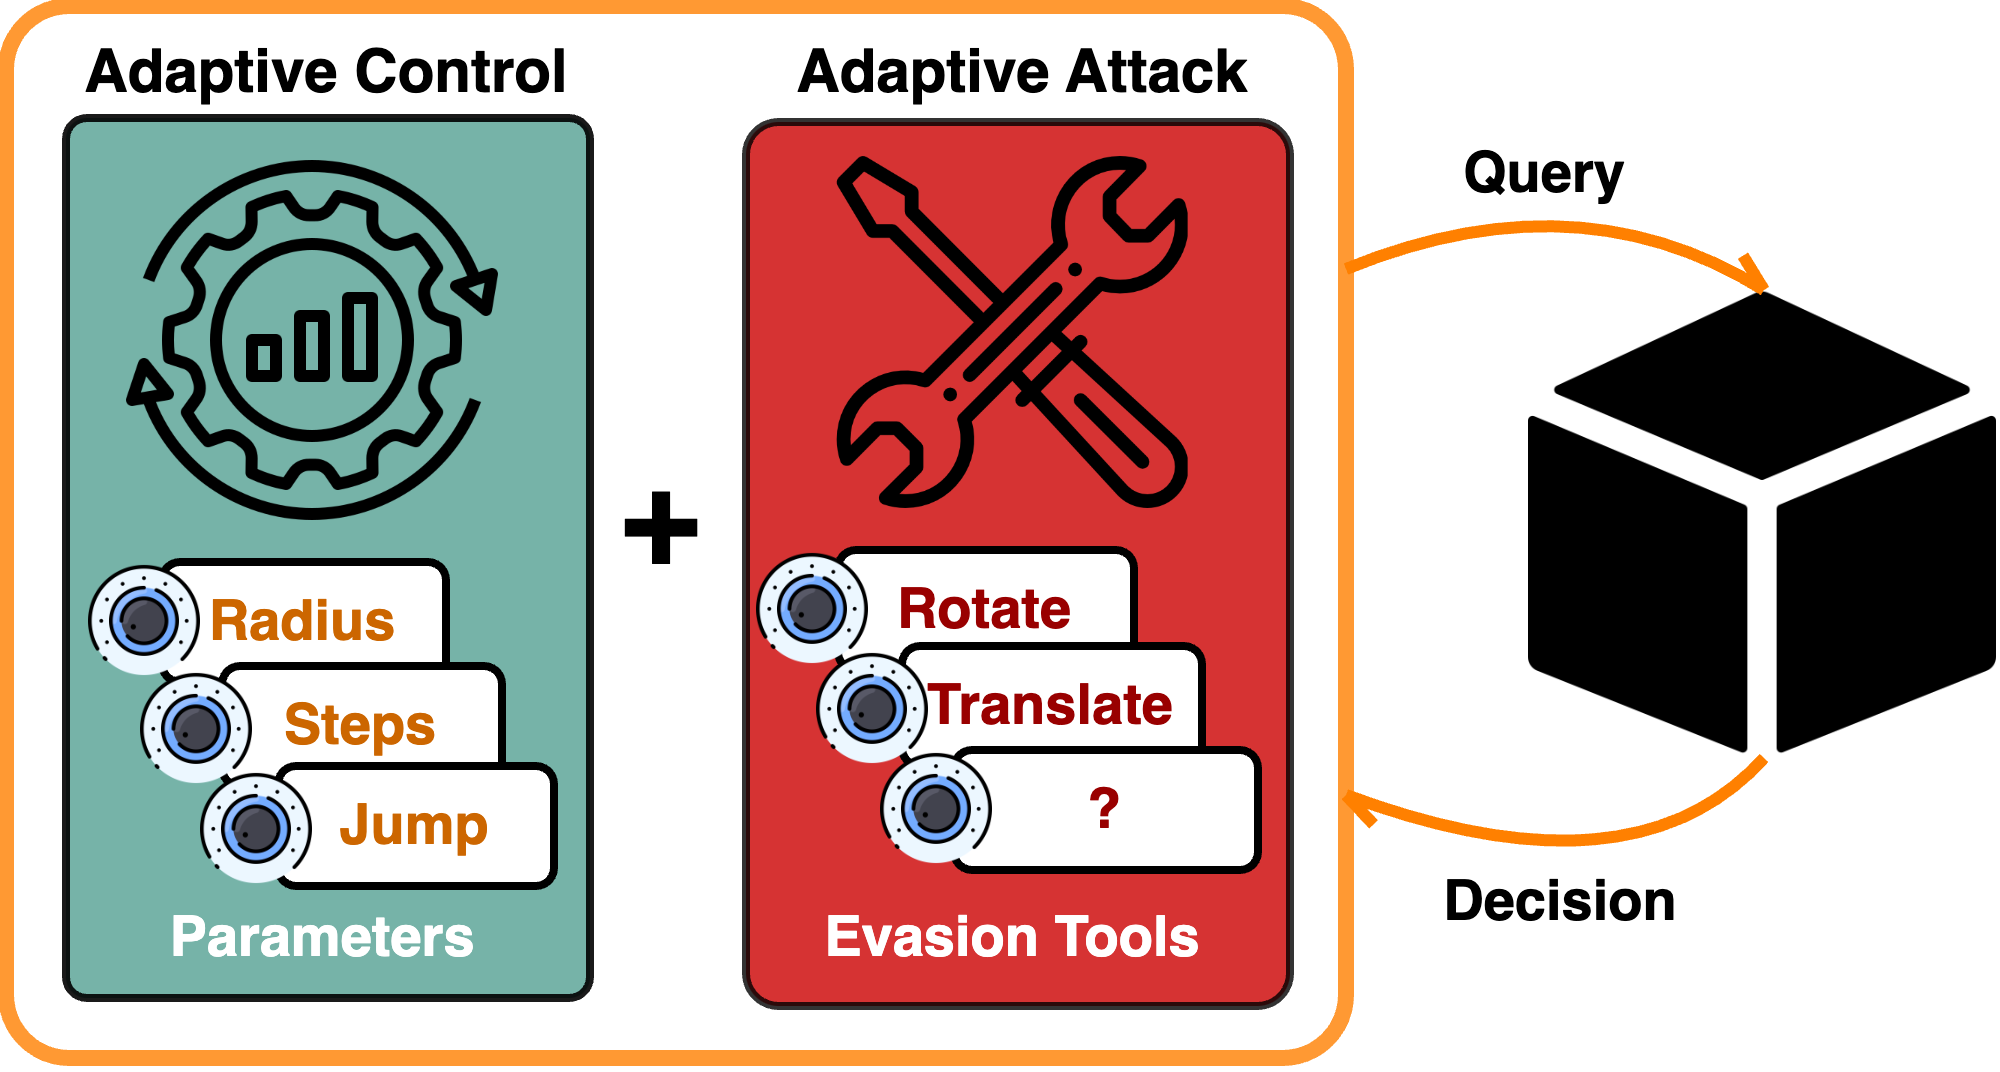
\includegraphics[width=0.9\textwidth]{knobs.png}
  \caption[Adaptive attacks reformulation.]{In \gls{AML}, adaptive attacks are those with the capabilities (knobs) to bypass a defense; adaptive control is rather the precise tuning of all the known knobs. Against black-box systems, we can reformulate adaptive so that it signifies \textbf{both}. For instance in HSJA~\cite{chen2020hopskipjumpattack}, radius, steps, and jump are parameters of the attack, while rotate and translate are transformations that can evade a similarity-based defense.}
  \label{fig:adaptivity}
\end{figure}

% the research gap
\subsection{Research Gap}
Prior work has focused on \textit{adapted} attacks, which incorporate general knowledge of any defenses and empirically configured to evade it~\cite{carlini2017towards, chen2020hopskipjumpattack, brendel2018decision}.
Defenses also follow the same adapted paradigm of empirically defined and fixed parameters~\cite{chen2020stateful, li2022blacklight}.
Our observation is that neither of them are formalized or performed in a fully adaptive manner, that is in response to how they influence their environment and with respect to other adaptive agents in it, with clear limitations when the latter is a given, e.g. in cybersecurity.
To bridge this gap, we provide a theoretical treatment and empirical study of existing and novel methodologies adapting through direct interaction with their environment, denoting them as \textbf{self-adaptive}.

Our work builds on a long line of prior research that focuses on both sides of the competition between adversaries and defenses.
\textbf{Carlini and Wagner}~\cite{carlini2017towards} show that evaluating existing attacks out-of-the-box is insufficient and that adapted white-box attackers can break defensive distillation.
\textbf{Bose et~al.}~\cite{bose2020adversarial} propose Adversarial Examples Games (AEG), a zero-sum game between a white-box attacker and a local surrogate of the target model family.
At the equilibrium the attacker can generate adversarial examples that have a high success rate against models from the same family, constituting a zero-query, non-interactive approach for generating transferable adversarial examples.
\textbf{Pal et al.}~\cite{pal2020game} propose a game-theoretic framework for studying white-box attacks and defenses that occur in equilibrium.
\textbf{Feng et al.}~\cite{feng2023stateful} introduce \textbf{OARS}: adaptive versions of existing attacks that bypass \textbf{Blacklight}~\cite{li2022blacklight}, the state-of-the-art stateful defense.
% \textbf{Ren et al}.~\cite{ren2021unified} explain adversarial robustness through low and high-order interactions between features.
% \textbf{Yasodharan et al}.~\cite{yasodharan2019nonzero} study adversarial classification by formulating it as non-zero-sum hypothesis testing game.
%Chen et~al.~\cite{chen2020stateful} introduce a stateful defense that leverages the interactive behavior of decision-based attacks (like Boundary Attack~\cite{brendel2018decision}) to detect and reject their queries.
To function, OARS presupposes the rejection signal that a defense like Blacklight returns; a strong assumption that as we show in this work does not have to hold for stateful defenses.
As we demonstrate in~\autoref{sec:evaluation} and~\autoref{tab:result3}, Blacklight can be bypassed without assuming rejection, while the novel stateful defense we introduce can fully withstand the OARS adaptive attack.

As the most relevant and representative threat against real-world AI systems, in this work we scope on decision-based, interactive attacks and defenses.
We contribute a theoretical and practical framework for self-adaptation, under which the full extent of the offensive and thus also the defensive potential is properly assessed.
In the remainder of the paper the term \textbf{``adaptive''} subsumes adaptive control, and is used interchangeably with \textbf{``self-adaptive''}.
For what is conventionally known as adaptive evaluations in \gls{AML}, we use the term \textbf{``adapted''}.
To facilitate comparison, in~\autoref{tab:comparison} we highlight the most important aspects of our work as the synthesis of adaptive black-box attacks and defenses in a unified framework, and situate it with respect to other relevant and state-of-the-art works in \gls{AML}.
Note the importance for an attack to function without assuming rejection, and respectively for a defense to function without access to query metadata like IP addresses or accounts.

\begin{table}[h]
\caption[Prominent decision-based attacks and defenses.]{Prominent decision-based attacks and defenses and their individual aspects: op=optimized, ev=evasive, aa=attack adaptation, $\neg$rj=doess not require rejection, ac=Active, ad=defense adaptation, $\neg$md=does not use metadata, ms=misdirection. While all works are situated either on the offensive or the defensive side, ours brings these two together.} 
\centering
\begin{tabular}{r|cccc|cccc}
\toprule
\multirow{2}{*}{\textbf{Work}} & \multicolumn{4}{c}{\textbf{\textcolor{purple!80}{Offensive}}} & \multicolumn{4}{c}{\textbf{\textcolor{teal!80}{Defensive}}} \\
\cmidrule{2-9}
& \textbf{op} & \textbf{ev} & \textbf{aa} & \textbf{$\neg$rj} & \textbf{ac} & \textbf{ad} & \textbf{$\neg$md} &\textbf{ms} \\
\midrule
\textbf{\textcolor{purple!80}{Boundary}}  \cite{brendel2018decision} & \emptycirc & \emptycirc & \emptycirc & \fullcirc & \emptycirc & \emptycirc & --- & --- \\
\textbf{\textcolor{purple!80}{BAGS}} \cite{brunner2019guessing} & \emptycirc & \emptycirc & \emptycirc & \fullcirc & \emptycirc & \emptycirc & --- & --- \\
\textbf{\textcolor{purple!80}{HSJA}} \cite{chen2020hopskipjumpattack} & \fullcirc & \emptycirc & \emptycirc & \fullcirc & \emptycirc & \emptycirc & --- & --- \\
\textbf{\textcolor{purple!80}{OARS}} \cite{feng2023stateful} & \fullcirc & \fullcirc & \halfcirc & \emptycirc & \fullcirc & \emptycirc & --- & --- \\
\midrule
\textbf{\textcolor{teal!80}{Adv. Train}} \cite{madry2017towards} & \fullcirc & \emptycirc & \emptycirc & --- & \emptycirc & \emptycirc & --- & ---\\
\textbf{\textcolor{teal!80}{Stateful}} \cite{chen2020stateful} & \fullcirc & \fullcirc & \emptycirc & \emptycirc & \fullcirc & \emptycirc & \emptycirc & \emptycirc \\
\textbf{\textcolor{teal!80}{Blacklight}}  \cite{li2022blacklight} & \fullcirc & \fullcirc & \emptycirc & \emptycirc & \fullcirc & \emptycirc & \fullcirc & \emptycirc \\
\midrule
\textbf{\textcolor{orange!80}{Our work}}  & \fullcirc & \fullcirc & \fullcirc & \fullcirc & \fullcirc & \fullcirc & \fullcirc & \fullcirc \\
\bottomrule
\label{tab:comparison}
\end{tabular}
\end{table}

\label{sec:approach}
To investigate the robustness to evasion of real-world systems, two closely related perspectives are pertinent: a) thwarting decision-based attacks, and b) adapting attacks and evasive capabilities \textit{in tandem}.
For the latter, when attacks (and defenses) are evaluated in a non-adaptive manner, in the expansive sense we outlined in \autoref{sub:adaptive}, results are rendered incomplete and untrustworthy~\cite{tramer2020adaptive, pintor2022indicators}.
Nevertheless, when offensive or defensive techniques adapt the environments that they inhabit become non-stationary~\cite{hernandez2017survey}, putting further pressure on the IID foundations that ML builds on.
To understand the implications of such techniques adapting, we perform a theoretical analysis of the possible interactions around the exposed interface of an ML-based system, interactions that can be more generally considered as sequential zero-sum games~\cite{littman1994markov, hardt2016strategic, bose2020adversarial}.
We initiate our analysis from adversaries, as the original factor and cause.

\subsection{Attacks}
The most compelling threat that deployed ML-based systems face are decision-based black-box attacks, where no access is assumed to the model or its parameters, only the capacity to submit queries and receive hard-label responses.
One of the first decision-based attacks was Boundary Attack~\cite{brendel2018decision}.
A large number of others followed -- each inventive in its own way -- that manage to improve the overall performance, typically measured as the lowest perturbation achieved for the minimal amount of queries submitted.
Prominent examples are HSJA~\cite{chen2020hopskipjumpattack}, Guessing Smart (BAGS)~\cite{brunner2019guessing}, Sign-Opt~\cite{cheng2019sign}, Policy-driven (PDA)~\cite{yan2020policy}, QEBA~\cite{li2020qeba}, and SurFree~\cite{maho2021surfree}.

White-box attacks like C\&W~\cite{carlini2017towards} cannot function in black-box environments as there is no closed-form description of the inference pipeline.
To facilitate optimization, decision-based attacks commonly initialize from a sample $x_g$ that belongs to the target class, as it can be considered an adversarial example with an unacceptably large perturbation.
This switch allows the task to be solved continuously, by minimizing the perturbation while always staying on the adversarial side of the boundary.
Decision-based attacks share further common aspects in their functioning, ones that we can abstract through: given \textbf{starting} and \textbf{original} samples $x_g$ and $x_c$ respectively, the goal is to iteratively propose adversarial \textbf{candidates} $x_t$, until the \textbf{distance} $\delta = d(x_t, x_c)$ is minimized (cf. Fig. \ref{fig:boundary}).
This process follows different algorithmic approaches that represent different geometrical intuitions; we can describe it more generally by means of a candidate generation policy:

\begin{equation}
    \pi_\theta^{\mathcal{A}} = P\: (x_{t}|x_g, x_{c}, p^{\mathcal{A}}, s^{\mathcal{A}})
\label{eqn:genpolicy}
\end{equation}

\noindent that given $x_g$ and $x_{c}$, with $p^{\mathcal{A}}$ the \textbf{parameters} and $s^{\mathcal{A}}$ the \textbf{state} of the attack, generates a candidate $x_t$.
% Such parameters are the source and orthogonal steps for BAGS and the number of queries and radius for the gradient approximation in HSJA.
If we consider that attacks execute over discrete time steps, and assume the model always answers, then the attack procedure can be construed as a \gls{MDP} to be solved, by finding the parameters $\theta$ that minimize $\delta$ in the least amount of queries.

%Scoping on image classification, we now introduce some necessary notation.
Consider now a multinomial image classification model $\mathcal{M}$ under attack, with a discriminant function $F: \mathbb{R}^d \rightarrow \mathbb{R}^m$, that for each input $x \in [0,1]^d$ generates an output $y := \{y \in [0,1]^m |\sum_{c=1}^{m}y_c = 1\}$ -- a probability distribution over the $m$ classes.
By definition, black-box environments preclude access to these probabilities; instead one can only observe the decision of the classifier $C$ that returns the highest probability class:

\begin{equation}
    C(x) := \operatorname*{arg\,max}_{c \in [m]} F_c(x) = D(F_c(x))
\label{eqn:classifier} 
\end{equation}

\noindent with $D$ being the decision function, here $D = \operatorname*{arg\,max}$.
The goal in targeted attacks is to change the \textbf{decision} $c_g \in [m]$ for a correctly classified example $x$, to a predefined \textbf{target} class $c_o \neq c_g$.
This process can be facilitated through a function $\psi$ which given a perturbed example $x_t$ at step $t$, it returns a binary indicator of success:

\begin{equation}
    \psi(x_t) = \begin{cases}
                    1 & \text{if}\quad C(x_t) = c_o\\
                    -1 & \text{if}\quad C(x_t) \neq c_o
                \end{cases}
\label{eqn:psi}
\end{equation}

As long as the model responds, $\psi$ can always be evaluated, it thus constitutes an essential mechanism upon which decision-based attacks build.
The adversarial goal can then be described as the following constrained optimization problem:

\begin{equation}
    \operatorname*{min}_{x_t} \: d(x_t,x_c) \quad \text{s.t.} \quad \psi(x_t) = 1,
\label{eqn:opt}
\end{equation}

\noindent where the distance metric $d$ is an $\ell_p$-norm, with $p \in \{0,1,2,\inf\}$.
As the threshold between adversarial and non-adversarial relies on the subjectivity of human perception, this optimization task highlights the fuzzy nature of adversarial examples, something that is further aggravated in domains where visual proximity is of little importance.
Successful or unsuccessful adversarial examples are therefore delimited by an \textbf{threshold} $\epsilon$ on perturbation, where $d(x,x_t) \leq \epsilon$.
While this constraint might not intuitively translate to non-visual domains, we nonetheless contend that minimal perturbation still remains a desideratum of adversarial examples.

The fact that real-world attacks are black-box and decision-based does not make them any less effective.
For instance, HSJA is guaranteed to converge to a stationary point of~Eq.~\eqref{eqn:opt}.
Given typical $\epsilon$ values for imperceptibility, this results in high attack success rates, even against \textit{adversarially trained} models. 
The limited effectiveness of adversarial training against decision-based attacks can be attributed to the fundamentally out-of-distribution (OOD) nature of adversarial examples, and the inherent challenges in the saddle point optimization problem in Eq.~\eqref{eqn:adv_train} that make it difficult for algorithms to converge to a global solution.
Additionally, decision-based attacks are challenging to incorporate during stochastic gradient descent (SGD) because these attacks rely on boundary navigation, and the farther the model is from convergence, the less effective the attack is.
Scalability is another concern: while adversarial training typically involves a few steps (1-50) of white-box attacks like FGSM or PGD, decision-based attacks can take orders of magnitude more steps (queries) to produce an adversarial example.

Decision-based attacks search for the \textbf{optimal parameters} $\theta^*$ of the generation policy \eqref{eqn:genpolicy}, those that given $x^{i}_{c}$, with $i$ denoting the i-th adversarial episode, minimize Eq.~\eqref{eqn:opt} in expectation:

\begin{equation}
    \operatorname*{arg\,min}_{\theta} \mathbb{E}[\sum_{i=1}^{N}d(x^i_b,x^i_c)], \quad \text{s.t.} \quad \psi(x^i_b) = 1,
\label{eqn:rew}
\end{equation}

\noindent where $x^i_b$ is the \textbf{best} adversarial example generated by policy $\pi_\theta^{\mathcal{A}}$ during episode $i$.
Given the dimensionality, it can be intractable to learn a policy that modifies the inputs at the feature space directly~\cite{pierazzi2020intriguing}; CIFAR-10, for instance, has more than 3K features to perturb.
%decision-based attacks have also a second objective to minimize: the number of queries submitted.

In AI-enabled systems, the best practice is to freeze the model after validation so that no novel issues are introduced by retraining: for all queries $x_t$ submitted during an attack session, we can therefore assume that $F_0 = F_1 = ... = F_t, \forall t$.
While this is representative of real-world settings, it is also what enables adversaries to discover adversarial examples that were not identified beforehand.
The fact however that adversaries follow a candidate generation policy, introduces a querying behavior which can be observed and exploited by a defensive methodology.
Consequently, while model-hardening approaches like adversarial training are \emph{necessary}, they can be \emph{insufficient} in defending from decision-based attacks.

\begin{proposition}
Let $F_c$ be the discriminant function of the adversarially trained model $\mathcal{M}$. Then in order for $\mathbb{E}[\sum_{i=1}^{N}d(x^i_b,x^i_c)] \geq \epsilon$ in HSJA, two capabilities are necessary: a) a decision function $D' \neq \operatorname*{arg\,max}$, and b) additional context $\tau$ s.t for adversarial query $x_t$, $C(x_t) = D(F_c(x_t)) \neq D'(\tau, F_c(x_t))$.
\label{prop:one}
\end{proposition}

Intuitively, HSJA operates in 3 stages which repeat: a binary search that puts $x_t$ on the decision boundary, a gradient estimation step, and projection step along the estimated gradient.
If the model \emph{always} responds truthfully, the adversary will be able to accurately perform all these steps and converge to the optimal adversarial; without loss of generality, we can extend this intuition to other decision-based attacks which navigate the boundary.
Secondly, the model should be able to differentiate between two, otherwise identical, queries when one is part of an attack and the other is not, and this is possible through a stateful representation; see Appendix~\ref{apx:proofs} for the proof.

\subsection{Defenses}

Proposition~\ref{prop:one} indicates that alternative classification policies are necessary in the presence of decision-based attacks, for instance classification with rejection or intentional misdirection.
In related work, rejection has been realized in the form of conformal prediction where model predictions are sets of classes including the empty one, or learning with rejection~\cite{barbero2022transcending, cortes2016learning}; while misdirection has emerged as a technique in adversarial RL and cybersecurity domains~\cite{gleave2020adversarial, sengupta2020multi}.
While adversarially training the discriminant function $F$ empirically shows the capacity to resist decision-based attacks, the manner in which the model responds has a complementary potential.
This gap between the empirical and theoretically possible robustness to decision-based attacks is the locus where a distinct from model hardening, active and adaptive defense can emerge.
Active defenses have direct implications on attacks themselves however.
Let us now assume an agent carrying out an \textbf{active defense policy}:

\begin{equation}
\pi_\phi^{\mathcal{D}} = P(\alpha_t|x_t,s^{\mathcal{D}}_t), \: \alpha \in \{0,1\}
\label{eqn:def}
\end{equation}

\noindent with $x_t$ the query, $s^{\mathcal{D}}_t$ the \textbf{state} for the defense as created by past queries, and $\alpha$ the \textbf{binary decision}: when the query is deemed adversarial, it is rejected by returning $\alpha=1$.
If this policy is stationary, the environment dynamics in turn become stationary too, and thus together with the adversarial task itself, bypassing the defense can \emph{also} be formulated as an MDP to be solved.
In two-player, zero-sum games, the moment an agent follows a stationary policy, it becomes \textit{exploitable} through the reward obtained by an adversary~\cite{timbers2022approximate}.
Active defenses, a consequence of decision-based attacks, entail therefore \textit{adaptive} adversaries.

\begin{proposition}
Against an active defense $\pi_\phi^{\mathcal{D}}$ and for time horizon $T$, a decision-based attack following a non-adaptive candidate generation policy $\pi_t = \pi_\theta^\mathcal{A}, \forall \: t \in [0,T]$ will perform worse in expectation \eqref{eqn:rew}, that is $\mathbb{E}[\sum_{i=1}^{N}d(x^i_b,x^i_c)]^{\mathcal{D}} > \mathbb{E}[\sum_{i=1}^{N}d(x^i_b,x^i_c)]^{\cancel{\mathcal{D}}}$.
\label{prop:two}
\end{proposition}

A proof for BAGS and HSJA is included in Appendix~\ref{apx:proofs}.
An adversary can reason, as a corollary to Proposition~\ref{prop:one}, that such defenses \emph{have to} be in place as it is suboptimal not too.
However, there is a second reason to consider adaptive attacks even in the absence of active defenses, as attack policies are often suboptimal with their default, empirically defined parameters.
Adapting attack policies is essentially the optimization of these parameters, and as an approach has proven very effective in other black-box or expensive-to-evaluate contexts, like Neural Architecture Search and Data Augmentation~\cite{zoph2016neural, pham2021autodropout, tsingenopoulos2024train}.
Our results in Section~\ref{sec:evaluation} further indicate the correspondence between adaptive and self-optimizing, showing that adaptive attacks consistently outperform non-adaptive, particularly against active defenses.

Consider now an active defense that is based on a similarity or a conformal metric.
In the twofold meaning we introduced in Section \ref{sec:background}, adaptive attack implies the \textit{capability} to bypass a similarity based defense; adaptive control implies optimization instead, the active tuning of all the available tools to evade the defense \textit{and} minimize the perturbation~(cf. Fig. \ref{fig:adaptivity}).
The revised adversarial objective then is to find the optimal policy that \emph{also} evades detection, and the way to achieve this is by adapting the candidate generation policy \eqref{eqn:genpolicy} itself.
Notably, and despite the black-box and discontinuous nature of the task, this optimization can be \emph{fully} gradient-based.
Decision-based attacks can recover \textbf{gradient-based} solutions to their objective, despite \emph{neither} the active defense \emph{nor} the model itself being accessible in closed-form.
For model $\mathcal{M}$, adversarial queries $x_t$, and active defense $\pi_\phi^{\mathcal{D}}$ making decisions $\alpha_t$, we can thus formulate the following:
% $\alpha_t = \pi_\phi^{\mathcal{D}}(x_t, s^{\mathcal{D}_t})$

\begin{proposition}[Adversarial Policy Gradient]
Given adversarial policy $\pi_\theta^\mathcal{A}$ \eqref{eqn:genpolicy} that generates episodes $\tau_i$ of queries $x_t$, and reward function $r(\tau_i) = \sum_{x_t \in \tau_i} (1 - \alpha_t)$, the optimal evasive policy ${\pi^\mathcal{A}_{\theta^*}}$ is obtained by gradient ascent on the policy's expected reward, $\nabla_\theta \mathbb{E}_{\pi_\theta^{\mathcal{A}}} [r(\tau_i)]$.
\label{th:epg}
\end{proposition}

%by updating $\theta$ in the direction of the


The proof is included in Appendix~\ref{apx:proofs}.
So far we have established that, \textbf{a)} in the presence of decision-based attacks, active defenses are necessary, yet conditional on adversarial agency they are insufficient and, \textbf{b)} adaptive attacks can become optimal in terms of both evasion and efficiency by observing and adapting to the discrete model decisions.
To complete the puzzle, the last piece is turning active defenses also adaptive.

\begin{corollary}
The active defense achieves its optimal $\pi_{\phi^*}^{\mathcal{D}}$~\eqref{eqn:def}, i.e. maximizing expectation $\mathbb{E}[\sum_{x_t \in \tau_i}P(\alpha_t|x_t,s^{\mathcal{D}}_t)]$, by adapting its policy against the optimal evasive policy ${\pi^\mathcal{A}_{\theta^*}}$.
\label{prop:3}
\end{corollary}

\begin{proof}
  As offensive and defensive policies are strictly competitive, we can define a reward $\rho$ of the defensive policy as $\rho(\tau_i) = \sum_{x_t \in \tau_i} \alpha_t$.
  Then by fixing the optimal evasive policy $\pi_{\theta^*}^\mathcal{A}$, and updating $\pi_\phi^{\mathcal{D}}$ with expected reward $\mathbb{E}_{\pi^\mathcal{D}_\phi}[\rho(\tau_i)]$ gradients, at convergence the resulting ${\pi^\mathcal{A}_{\theta^*}}$ will be the optimal defensive policy.
  \end{proof}

\begin{figure}
    \centering
    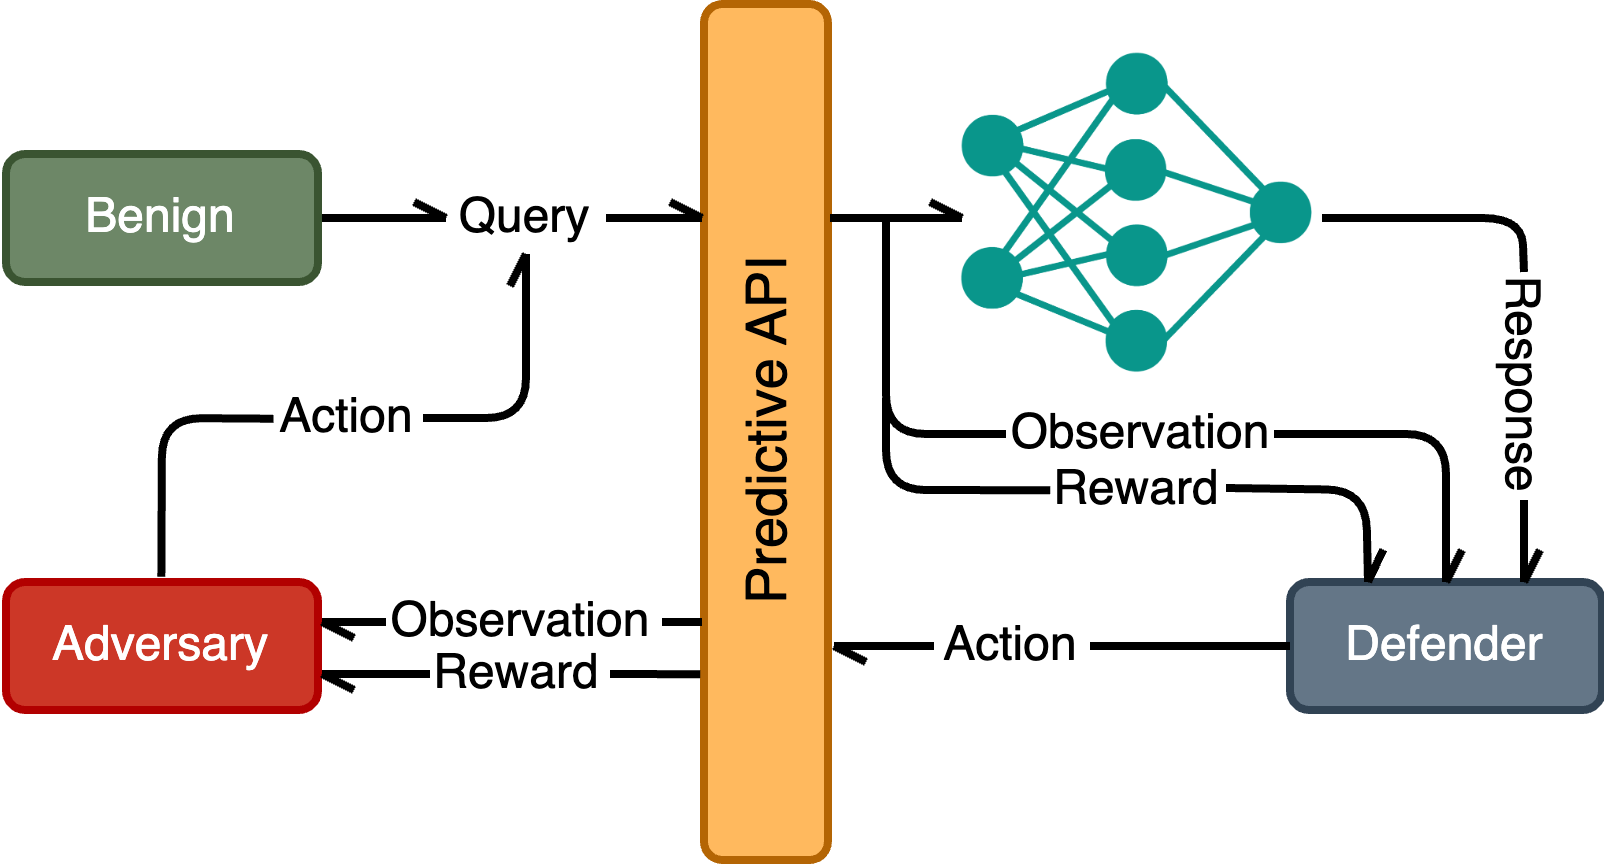
\includegraphics[width=0.9\textwidth]{model.png}
    \caption[Schematic model of an AMG environment.]{Schematic model of an AMG environment. Due to the inherent uncertainty of behavior at either side of the interface, it is a partially observable RL environment mirrored for each agent where one's decisions become the other's observations. (I) denotes an adaptive attacker (cf. Fig. \ref{fig:adaptivity}), (II) model hardening (passive defense), and (III) an active defense.}
    \label{fig:model}
\end{figure}

\subsection{Adversarial Markov Games}
\label{sec:AMG}

By reasoning on both offensive and defensive capabilities, we highlighted why we cannot consider them independently from each other.
As adaptive decision-based attacks and defenses are logical consequences of each other, by composing them we can form a turn-taking competitive game.
A precise game-theoretic formulation requires the exact analytical description of the whole environment: the model, the players and their utility functions, as well as the permitted interactions and the transition dynamics, something exceedingly intractable in this context as well as most cybersecurity environments.
Model-free methods however can learn optimal offensive and defensive responses directly through interaction with the environment~\cite{sengupta2020multi, schulman2017proximal}, obviating the need to learn a model of it or to find \emph{exact} solutions the to bi-level optimization task like Eq.~\eqref{eqn:adv_train} that is inherently NP-hard to solve~\cite{bruckner2011stackelberg}.

To that end, Turn-Taking Partially-Observable Markov Games (TT-POMGs) introduced by Greenwald et al.~\cite{greenwald2017solving} is a generalization of Extensive-Form Games (EFGs), widely used representations for non-cooperative, sequential decision-making games of imperfect and/or incomplete information; an apt formalism for decision-based attacks and defenses.
Another nice property of TT-POMGs is that they can be transformed to equivalent belief state MDPs, significantly simplifying their solution.

The competition underlying adversarial example generation has been explored in no-box and white-box settings~\cite{bose2020adversarial, gao2022achieving}.
We instead focus on decision-based, interactive environments which are assumed to have unknown but stationary dynamics: any agency present is considered part of the environment and therefore fixed in its behavior.
By folding the strategies of other agents into the transition probabilities and the initial probability distribution of the game, an optimal policy computed in the resulting MDP will correspond to the best-response strategy in the original TT-POMG.
The congruence between TT-POMGs and MDPs is useful not only from a theoretical perspective, but also for its practical implications in the security of ML-based systems: provided that adversarial agents and their capabilities can be identified through rigorous threat modeling, computing the best response strategy in the simulated environment will correspond to the optimal defense.
%It is safe to assume that if other agents inhabit the environment, then at the time of learning a best response they employ stationary policies.
% refer to discovering agents here

This environment that encompasses adversarial attacks, adversarial defenses, and benign queries, can be construed as an Adversarial Markov Game (AMG) -- a special case of TT-POMG -- and is depicted in Figure~\ref{fig:model}.
Formally, we represent AMG as a tuple $\langle i, S, O, A, \tau, r, \gamma \rangle$
\begin{itemize}
    \item $i = \{\mathcal{D}, \mathcal{A}\}$ are the players, where $\mathcal{D}$ denotes the defender and $\mathcal{A}$ denotes the adversary. In our model, benign queries are modeled as moves by nature.
    \item $S$ is the full state space of the game, while $O = \{O^{\mathcal{D}}, O^{\mathcal{A}}\}$ are partial observations of the full state for each player.
    \item $A = \{A^{\mathcal{D}}, A^{\mathcal{A}}\}$ denotes the action set of each player.
    \item $\tau(s,a^{i},s')$ represents the transition probability to state $s' \in S$ after player $i$ chooses action $a^i$.
    \item $r = \{r^{\mathcal{D}}, r^{\mathcal{A}}\} : O^i \times A^i \rightarrow \mathbb{R}$ is the reward function where $r^i(s, a^i)$ is the reward of player $i$ if in state $s$ action $a^i$ is chosen.
    \item $\gamma^i \in [0,1)$ is the discount factor for player $i$.
\end{itemize}

The goal of each player $i$ is to determine a policy $\pi^{i}(A^i | O^i)$ that, given the policy of the other(s), maximizes their expected reward.
When a player employs a stationary policy, the AMG reduces to a belief-state MDP where the other interacts with a fixed environment.
The game is sequential and turn-taking, so each player $i$ chooses an action $a$ from their set of actions $A^i$ which subsequently influences the observations of others.
%In Chapter~\ref{sec:threat} and Appendix~\ref{apx:rew} we elaborate on the concrete definitions of states, actions, and rewards that we conducted our empirical evaluations with.

We have shown that an adaptive defense policy $\pi^{\mathcal{D}}_\phi$ is necessary to deter decision-based attacks, and as a consequence the candidate generation policy $\pi^{\mathcal{A}}_\theta$ has to be adaptive in turn.
%These policies, parameterized by $\phi$ and $\theta$ respectively, are learned on the observations from each agent perspective.
As without implausible assumptions one cannot assume access to the exact state of the other agent, the states $O^{\mathcal{D}}$, $O^{\mathcal{A}}$ are partial observations of the complete state $\mathcal{S}$ of the full game.
When human agents compete by holding beliefs about each other, they engage in recursive reasoning that in theory of mind is encountered as [I believe that [my opponent believes [that I believe...]]].
In the study of opponent modeling, considering other agent policies as stationary and part of the environment is equivalent to \textit{0th} level recursive reasoning:
the agent models how the opponent behaves based on the observed history, but \emph{not} how the opponent \emph{would} behave based on how the agent behaves~\cite{albrecht2018autonomous, wen2019probabilistic}.
However, as AMGs can be solved by single-agent RL algorithms, we consider more involved recursive reasoning out of scope and perform the empirical evaluation without building explicit models of opponent behavior.

\section{Environment Specification}
\label{sec:threat}

The empirical study we conduct in Section~\ref{sec:evaluation} reflects diverse instantiations of the general theoretical framework introduced in Section~\ref{sec:approach}.
When working forward from the theoretical to the practical, concrete design choices have to be made when specifying the latter, choices that can have considerable influence on the results.
To elucidate our proposed robustness evaluation methodology, in this section we provide the concrete details on the threat model and the environment.

\textbf{[Threat Model].} Our AMG framework describes a two-player competitive game; while extensible to more players, in this work we assume that at a given moment only one attack takes place.
From the defensive perspective, incoming queries can be either benign or part of an attack.
An assumption that influences the effectiveness of stateful detection is that queries can be attributed to UIDs, e.g., an IP address or a user account.
However, adversaries can collude, create multiple accounts, use VPNs, or in fact accounts and IP addresses might not even be required to query the model.
To address this, we treat queries irrespective to their source.
This is a strictly more challenging setting for stateful defenses, where we operate solely on the content of queries and not on any other metadata, similar to~\cite{li2022blacklight}.
Unlike Blacklight however, instead of rejecting queries, something that by itself can provide \textit{more} information to the adversary and thus facilitate evasion (cf. OARS \cite{feng2023stateful}, \autoref{tab:comparison}), we misdirect by returning the second highest probability class.
Furthermore, Gaussian noise is added to the benign queries to simulate a noisy channel and a shift in distribution and so that is not trivial for a defense to tell adversarial noise apart.
In summary, the black-box threat model we consider is delineated as follows:

\begin{itemize}
    \item \textbf{Assets:} Trained and deployed model $\mathcal{M}$ with corresponding weights ${w}$.
    \item \textbf{Agents:} Adversary / Defender / Benign user.
    \item \textbf{Adversary Goal:} Generate minimal perturbation adversarial examples in as few queries as possible, while evading the defense.
    \item \textbf{Defender Goal:} Stop the adversary from generating adversarial examples, while preserving the correct functionality of the model $\mathcal{M}$ on benign users.
    \item \textbf{Adversary Knowledge:} The model $\mathcal{M}$ is known as the black-box function that transforms inputs $x \in [0,1]^d$ to outputs $c \in [m]$, $m$ being the number of classes. The weights ${w}$ and the closed-form expression of $\mathcal{M}$ are unknown, as unknown is if an active defense $\pi_\phi^{\mathcal{D}}$ exists or not.
    \item \textbf{Defender Knowledge:} The defender observes only the content of incoming queries, without knowing if they come from a benign user or the adversary.
    \item \textbf{Adversary Capabilities:} Adapt the parameters of the attack and optionally any evasive transformations; in essence, optimize the candidate generation policy $\pi^{\mathcal{A}}_\theta$.
    \item \textbf{Defender Capabilities} For each query $x$, decide between answering truthfully with the true prediction $C(x) = c_T$ or misdirect with the second highest probability class $c_S$.
\end{itemize}

\begin{figure}
    \centering
    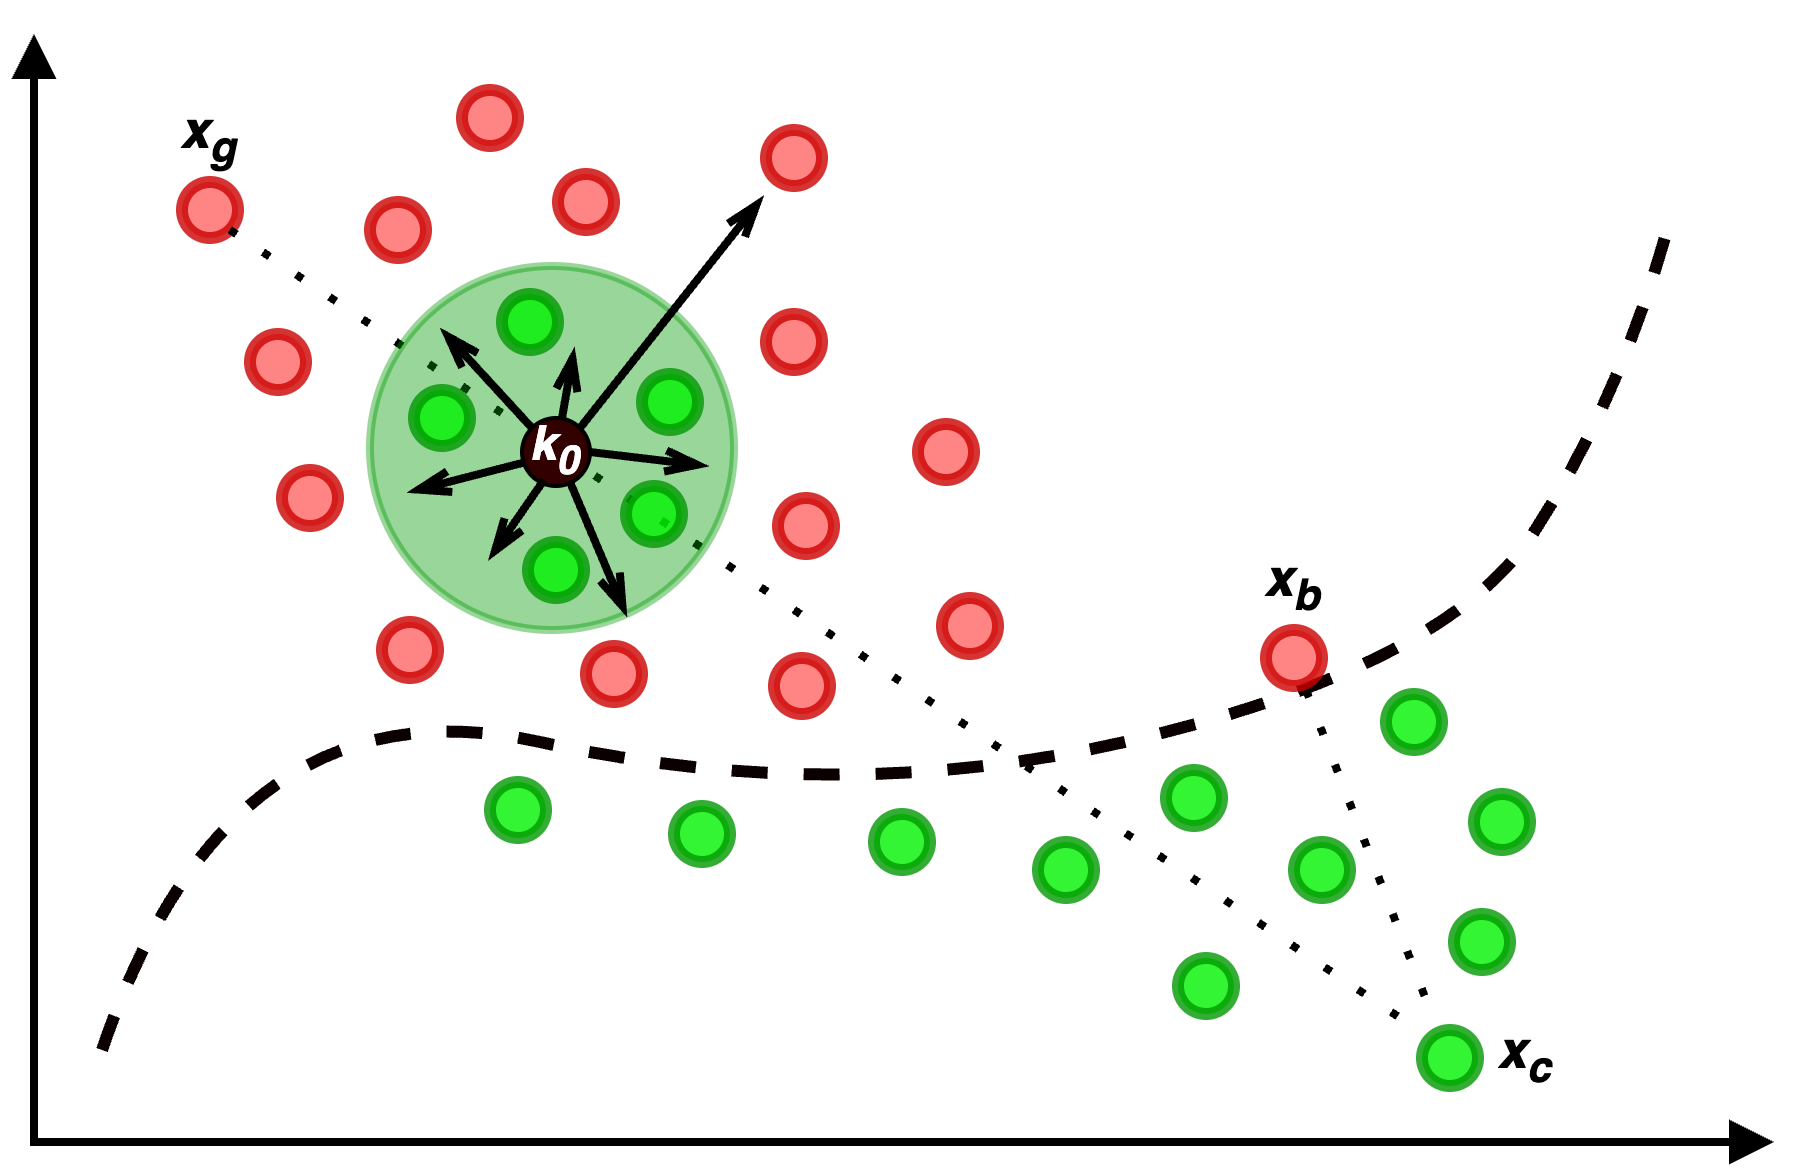
\includegraphics[width=0.9\textwidth]{boundary.png}
    \caption[Misdirection in a two-dimensional decision boundary.]{Misdirection in a two-dimensional decision boundary. The adaptive defense controls a single parameter, the hypersphere radius around $k_0$ (the last known adversarial); for queries $x_t$ that fall within this hypersphere the model responds with a non-adversarial decision. $x_g$ is the starting sample, $x_c$ the original, and $x_b$ the best possible adversarial.}
    \label{fig:boundary}
\end{figure}
% \vspace{-20pt}

\textbf{[Similarity].} Decision-based attacks typically follow a policy that generates successive queries: these exhibit degrees of similarity which can be quantified by an appropriate $l_p$ norm.
If that norm is computed on the original inputs however, an adversary can \textit{adapt} (see \autoref{fig:adaptivity}) by employing evasive transformations the model is invariant to and bypass the similarity detection.
To account for this capability, we train a Siamese network with contrastive loss in order to learn a latent space $\mathcal{L}(\cdot)$ where similar inputs are mapped close together, unaffected by added noise or transformations on the inputs.
%In the work of Chen et al. ~\cite{Chen} the choice of the detection threshold is done in such a manner that false positives are minimized. This threshold is set in advance to allow for a 0.1\% false positive rate. The comparative advantage an adaptive approach has is that there is no explicit and immediate need to set a threshold. The agent based on the current belief state and the level of uncertainty can opt for a less harsh action, like model swapping, or a more pronounced action, like returning the second highest confidence class when it is more confident that the query is part of an attack.
For the stateful characterization of queries, we use two queues: one for the detected adversarial queries as determined by the defensive agent, and one for the benign or undetected ones.
%We have to note at this point that the efficacy of the defense depends the continuous detection of adversarial queries so they are appointed to the correct queue and a representative state is constructed thereby.

\textbf{[Active defense].} Recall that decision-based attacks evaluate a Boolean-valued function to determine if the query is adversarial or not; a straightforward counter to this behavior is to misdirect by returning a decision different from the actual through a system of confinement.
%responding not with the actual class, i.e., the highest probability one, but the second highest.
When new query $x_t$ is received, a state is constructed based on $x_t$ and the queue $k_{-n}, k_{-n-1}, ..., k_{0}$ of known adversarial queries.
Based on this state, the defensive agent takes a single continuous action $\{\alpha \in \mathbb{R} \,|\, 0\leq \alpha \leq1\}$, with $\alpha$ being the radius of a hypersphere centered on the last known adversarial query $k_0$ in the latent space $\mathcal{L}$.
If $\|\mathcal{L}(x_t) - \mathcal{L}(k_0)\|_2 < a$ the query is considered adversarial and is appended to the adversarial queue as the latest $k_0$.
%If the $l_2$ distance between the embeddings of $x_t$ and $c_0$, $d(\mathcal{L}(x_t), \mathcal{L}(c_0))$, is within this radius $a$, the query is considered adversarial and is appended to the adversarial queue as the latest $c_0$.
This system of confinement is depicted in Figure~\ref{fig:boundary}.

\textbf{[Adaptivity].} No evaluation in \gls{AML} is complete without considering adaptive adversaries; a notion we expand in this work, that is with the instruments to bypass the defense \textit{and} their optimal configuration.
%that is without knowledge of the defense and its principle of operation, leaving out maybe the precisely \textit{how} to bypass it \cite{tramer2020adaptive}.
%Adaptive adversaries imply the invention of control:
As stateful defenses are so far similarity based, to bypass them intuition points towards input transformations the model is invariant to.
For a given query $x_t$ we want to compute a transformation $x_t' = T(x_t)$ so that $||x_t' - x_t||_2 \gg ||x_t - x_{t-1}||_2$ while $F(T(x_t)) \approx F(x_t)$.
Depending on magnitude and composition of transformations $T$, the identity $F(T(x_t)) = F(x_t)$ might not always hold.
As we also demonstrate in Section \ref{sec:evaluation}, $T$ interferes with the perturbations the adversarial policy generates itself: the performance and evasiveness of an attack are thus in a natural trade-off.

At this point we should inquire what is the correct composition of transformations $T$ to apply.
When shall $T$ be applied, and how does it affect the attack fundamentals?
The transformations $T$ can be considered as a set of additional controls, and like attack parameters they themselves can be suboptimal out-of-the-box \cite{croce2020reliable}.
Thus the combined control of attack and evasion parameters is a \emph{prerequisite} to properly assess the strength of a defense.
% their empirical configuration is often suboptimal against a particular defense and a fine balance is often required between evasion and preserving attack performance.
Their trade-off illustrates why the twofold definition of adaptive is necessary in \gls{AML} evaluations: first to impart the tools to accomplish to the task through the definition of \textit{what} can be controlled, and then to find the precise optimal configuration and strategy of the attack.

\textbf{[Agents \& Environments].} Unlike common competitive games, in AMGs the two players have different action and state sets.
AMGs are also asymmetric in the playing cadence: while the defender plays every round, the adversary might wait one to several rounds; HSJA for example is controlled on the iteration rather on the query level.
Training is complicated further given that the experience upon which each agent learns arrives only \emph{after} the opponent moves.
We address these complications by developing custom learning environments for agents with asymmetries, with delayed experience collection, and asynchronous training, build with the OpenAI Gym and Stable-Baselines3 libraries.
% ~\cite{brockman2016openai, raffin2019stable}.

\textbf{[States \& Actions]}. 
For the definition and the rationale behind the states we use, we point the reader to Appendix~\ref{apx:rew}.
For actions, we control BAGS through 4 parameters: orthogonal step size, source step size, mask bias, and Perlin bias.
HSJA is controlled by 3: the gradient estimation radius, the number of estimation queries, and the jump step size.
All evaluations start from controlling these attack parameters \textit{only}; if the active defense proves impossible to defeat, we introduce additional knobs that control the magnitude and probability of transformations on the input, with the goal to evade detection \emph{while} preserving semantic content and hence the correct classification.
The range of transformations we experimented with as well as their magnitude and probability are listed in~\autoref{tbl:transforms}.
Finally, in both BAGS and HSJA the active defense consists of an 1-dimensional continuous action that controls the radius of confinement $a$, as depicted in Fig~\ref{fig:boundary}.

\textbf{[Rewards]}. Success in an \gls{RL} task relies heavily on \emph{how} it is rewarded.
Engineering an effective reward function is non-trivial and hides intricacies, as reward hacking and specification gaming are common phenomena and the learned behavior can vary~\cite{amodei2016concrete}.
For adversaries, the rewards we experimented with are variations on minimizing the distance to the original example -- with extra reward shaping based on the fundamental operation of each attack -- while defenders are rewarded or penalized for intercepting adversarial or benign queries respectively.
% For BAGS, terms include the distance gains towards the original example (also relative to the initial gap) and on their frequency.
% For HSJA, additional terms include penalties for the amount of gradient estimation queries, and rewards on the precision of gradient estimation and jump steps.
% Defensive rewards for BAGS include keeping the best adversarial or the average query close to the starting point, minimizing the size of the step, and correctly intercepting queries.
% For HSJA, additional terms include penalties for not intercepting queries at the binary search or jump steps.
The rewards are described in Appendix~\ref{apx:rew}.

\section{Evaluation}
\label{sec:evaluation}
% As the empirical counterpart of our theoretical investigation, we perform an extensive evaluation by defining a range of scenarios that reflect all possible and realistic combinations between adversarial attacks and defenses.
For evaluation, we define a range of scenarios intended to reflect all possible and realistic combinations between adversarial attacks and defenses, and their adaptive versions.
Concretely, the research questions we want to validate are: 1) Are active defenses a necessary complement to model hardening and to what extent? 2) Are attacks more threatening when adaptive, i.e., do they outperform their vanilla versions \textit{and} evade active detection? 3) If yes, can active defenses recoup their performance by also turning adaptive?

\textbf{[Metrics]}. We employ \textbf{ASR} (Attack Success Rate) and $\mathbf{L_2}$ \textbf{norm} of the perturbation.
For the former we set a fixed threshold of 3 for consistency between experiments, while the latter is a more fine-grained metric well suited for comparing baseline attacks, defenses, and their adaptive versions, as it is not based on an (arbitrary) perceptual threshold that can yield widely varying results when moved.
The budgets we evaluate over are 1K, 2K and 5K queries.
As robustness and classification accuracy are typically in trade-off, the third metric of interest is the benign sample accuracy (\textbf{Clean Acc.}) that the original model and the active defense achieve together.

\subsection{Evaluation Setup}
Our goal is to learn offensive or defensive policies that are \emph{general}: they transfer to \textit{any} other evasion task.
Thus after training and validating the agents, the final performance is reported on a fixed hold-out set of 100 adversarial episodes where the starting and original samples are selected at random.
As is best practice in \gls{AML}, candidate samples are only those that are correctly classified by the model.
For each scenario we perform a hyperparameter and reward function exploration (max 30 trials), with the intention to root out poor combinations rather than exhaust the search space, described in detail in Appendix~\ref{apx:hyper}.

The black-box attacks we render adaptive and evaluate are \textbf{BAGS} and \textbf{HSJA}, as they represent two fundamentally different approaches, are highly effective, \emph{and} have the highest evasion potential \cite{li2022blacklight}.
BAGS is a stochastic, search-based method where every query submitted is a new and potentially better adversarial example.
Contrastively, HSJA is deterministic and composed of 3 different stages where the queries are generated in an aggregated manner: the vast majority of them are not candidate adversarial examples but means to approximate the gradient at the decision boundary.

In training and evaluation, the adversarial game is played as follows: the adversary starts by submitting a query, then the defender responds either \emph{truthfully} (the true model prediction) or by \emph{misdirecting} (the second highest probability class).
Then the environment decides with chance $p$ if the adversary moves next, otherwise a benign query is drawn.
In either case, it is the defender's turn; in testing they are also oblivious to the nature of the query and know only the content.
All experiments are performed with $p=0.5$; we also evaluate our trained defense when no attack is present ($p=0$) in Appendix~\ref{baserate}.

%For a wide and representative evaluation, we construct such scenarios for all possible combinations of (non-) adaptive attacks and defenses.
The scenarios for all possible combinations of (non-) adaptive attacks and defenses are repeated over two different datasets -- CIFAR10 and MNIST -- and over two models with the same architecture but with different training regimes: one with adversarial training and one without.
The transition from single-agent to multi-agent \gls{RL} hides challenges: we approach the AMG as a belief-state MDP (the requirement of knowing the exact opponent policies is relaxed) and use PPO \cite{schulman2017proximal} agents to discover optimal policies that will also constitute best responses for the full AMG~\cite{wen2019probabilistic}.
However, learning independently of other agency breaks the theoretical guarantees of convergence~\cite{tuyls2012multiagent}, eg. in scenarios 7 \& 8 where both agents learn simultaneously.
% this can be observed in the sole scenario where both agents learn simultaneously and we thus report them separately: 7 \& 8 AA-AD.
The complete list of scenarios is:

\begin{enumerate}[leftmargin=*]
  \setcounter{enumi}{-1} 
      \setlength\itemsep{0.1em}
      \item \textbf{VA-ND} -- Vanilla Attack / No Defense: Baseline performance of attacks (BAGS \& HSJA) out-of-the-box, without any active defense.
      \item \textbf{AA-ND} -- Adaptive Attack / No Defense: How more optimal is the adaptive version of an attack compared to the baseline.
      \item \textbf{VA-VD} -- Vanilla Attack / Vanilla Defense: The performance of our active defense, the non-adaptive version that has an empirically defined detection threshold.
      \item \textbf{AA-VD} -- Adaptive Attack / Vanilla Defense: Similar to scenario (2), but now the attack is adaptive.
      \item \textbf{VA-AD} -- Vanilla Attack / Adaptive Defense: The first scenario where the active defense is also adaptive, against the baseline adversary.
      \item \textbf{AA-TD} -- Adaptive Attack / Trained Defense: After the adaptive defense is optimized, its policy is fixed and an adaptive attack is trained against it.
      \item \textbf{TA-AD} -- Trained Attack / Adaptive Defense: The best policy found in the previous scenario is fixed and an adaptive defense is trained against it.
      \item \textbf{AA-AD} -- Adaptive Attack / Adaptive Defense: The first scenario where both agents learn simultaneously, making the environment non-stationary. In practice, the convergence will vary and depend on the chosen hyperparameters and rewards. Here we report the best-case for the attack.
      \item \textbf{AA-AD} -- Adaptive Attack / Adaptive Defense: The exact setup as scenario 7, but the best-case for the defense is reported instead.
  \end{enumerate}

For each successive scenario we evaluate with the most successful policy found, as this is best practice in Markov Games: the worst case opponent policy is fixed and then a counter to it is learned~\cite{littman1994markov, timbers2022approximate}.
Fixing other policies when computing a best response is representative of learning in cybersecurity environments that can contain a range of agents, with the additional benefit of converting the problem to single-agent that, as detailed in Section~\ref{sec:AMG}, one can solve with \gls{RL}.

\textbf{Comparison to state-of-the-art.} In Scenarios 0-8 we evaluate all possible combinations between our attack and our defense.
As a baseline to compare to, we additionally evaluate our approach to the state-of-the-art stateful defenses and adaptive attacks, that is Blacklight \cite{li2022blacklight} and OARS \cite{feng2023stateful} respectively.
We implement both Blacklight and OARS in our interactive environments by using their publicly available code and parameters.
As our environments do not return a rejection signal and to make a fair comparison, for OARS rejection coincides with a non-adversarial decision.
We define 5 further scenarios:

\begin{enumerate}[leftmargin=*]
\setcounter{enumi}{8} 
    \setlength\itemsep{0.1em}
    \item \textbf{VA-BD} -- Vanilla Attack / Blacklight Defense: Baseline performance of the attacks against Blacklight.
    \item \textbf{OA-BD} -- OARS Attack / Blacklight Defense: OARS against Blacklight.
    \item \textbf{AA-BD} -- Adaptive Attack / Blacklight Defense: Our adaptive attack against Blacklight.
    \item \textbf{OA-TD} -- OARS Attack / Trained Defense: OARS against our trained defense from Scenario 6.
    \item \textbf{OA-AD} -- OARS Attack / Adaptive Defense: Our adaptive defense retrained against OARS.
\end{enumerate}

Our experiments were run on multiple machines, however to give an idea for the time complexity of our defense, on an Intel i7-7700 CPU one forward pass in CIFAR -- that is one response to one query -- takes $8 \pm 1.4$ ms for 700 MFLOPs.

\subsection{Results}
For consistency and comparability between evaluations, all results are from the \emph{same} 100 test episodes.
The \textbf{gap} value denotes the $\ell_2$ perturbation that initially separates the starting and best adversarial example, averaged over the 100 episodes. 
% A perfect defense would therefore acquire a value very close to the gap, while a perfect attack would never be able to reduce the perturbation to $0$.
%it can be evaluated, however, relative to the baseline or other attacks.
By testing the trained agents on budgets higher than 5K we discovered that the trend in reducing $\ell_2$ holds; to make the agent training tractable and the evaluation wider however, we limit the maximum query budget per adversarial episode to 5K.
For CIFAR-10, tables~\ref{tab:BAGS_result} \& \ref{tab:HSJA_result} report the results on our adaptive agents as well as the state-of-the-art, for BAGS and HSJA respectively; tables~\ref{tab:BAGS_resultM} \& \ref{tab:HSJA_resultM} report the results for the MNIST dataset. 
% The color gradient ranges from the gap value to the minimum value that can be achieved @ 5K queries.
The empirical results, as yielded by months of CPU hours and an inordinate amount of trips to the whiteboard, help us extract several important insights, practical observations, and general implications for the broader \gls{AML} field:

\begin{table*}[!ht]
\setlength{\tabcolsep}{0.3cm} % Adjust column spacing here
\centering
  \caption[ASR and mean $l_2$ perturbation for BAGS in CIFAR-10.]{\textbf{CIFAR-10 / BAGS}: ASR and mean $l_2$ perturbation for 1K, 2K, and 5K queries, against normally and adversarially trained models. C.Acc reports the clean accuracy on benign queries of the base model plus any defenses present; in the first two scenarios (no active defense) the baseline clean accuracy is reported. Yellow scenarios denote the baseline attack performance, green denote active and/or adaptive defenses, and red denote adaptive attacks. Scenarios 9-13 compare our Adaptive Attack (AA) and Adaptive Defense (AD) to Blacklight (BD) and OARS (OA).}
  \begin{tabular}{c|c|rrrr|r}
    \toprule
      \multirow{2}{*}{\parbox{1cm}{\centering Adv.\\Trained}} & \multirow{2}{*}{Scenario} & \multicolumn{5}{c}{\textbf{CIFAR-10 Gap: 20.01}} \\
      & & {1K} & {2K} & {5K} & {ASR} & {C.Acc} \\
      \toprule
    \multirow{14}{*}{\xmark} & \raggedright\textbf{\textcolor{orange!70}{\phantom{*}0: VA-ND}} & 8.27 & 7.86 & 7.26 & \textcolor{t5!100}{\textbf{5\%}} & 91.69 \\
    & \raggedright\textbf{\textcolor{purple!70}{\phantom{*}1: AA-ND}} & 1.26 & 0.71 & 0.49 & \textcolor{t100!100}{\textbf{100\%}} & 91.69 \\
    & \raggedright\textbf{\textcolor{teal!70}{\phantom{*}2: VA-VD}} & 15.27 & 15.26 & 15.20 & \textcolor{t0!100}{\textbf{0\%}} & 91.68 \\
    & \raggedright\textbf{\textcolor{purple!70}{\phantom{*}3: AA-VD}} & 2.63 & 2.03 & 1.77 & \textcolor{t93!100}{\textbf{93\%}} & 91.69 \\
    & \raggedright\textbf{\textcolor{teal!70}{\phantom{*}4: VA-AD}} & 20.01 & 20.01 & 20.00 & \textcolor{t0!100}{\textbf{0\%}} & 91.60 \\
    & \raggedright\textbf{\textcolor{purple!70}{\phantom{*}5: AA-TD}} & 6.28 & 5.45 & 4.52 & \textcolor{t30!100}{\textbf{30\%}} & 91.52 \\
    & \raggedright\textbf{\textcolor{teal!70}{\phantom{*}6: TA-AD}} & 19.52 & 19.40 & 18.95 & \textcolor{t0!100}{\textbf{0\%}} & 91.38 \\
    & \raggedright\textbf{\textcolor{purple!70}{\phantom{*}7: AA-AD}} & 9.95 & 9.80 & 9.80 & \textcolor{t5!100}{\textbf{5\%}} & 91.66 \\
    & \raggedright\textbf{\textcolor{teal!70}{\phantom{*}8: AA-AD}} & 19.85 & 19.85 & 19.85 & \textcolor{t0!100}{\textbf{0\%}} & 91.69 \\
    \cline{2-7}
    & \raggedright\textbf{\textcolor{orange!70}{\phantom{*}9: VA-BD}} & 9.55 & 9.32 & 9.17 & \textcolor{t0!100}{\textbf{0\%}} & 91.71 \\
    & \raggedright\textbf{\textcolor{purple!70}{10: OA-BD}} & 9.46 & 9.46 & 9.46 & \textcolor{t1!100}{\textbf{1\%}} & 91.71 \\
    & \raggedright\textbf{\textcolor{purple!70}{11: AA-BD}} & 2.26 & 1.39 & 1.32 & \textcolor{t98!100}{\textbf{98\%}} & 91.71 \\
    & \raggedright\textbf{\textcolor{teal!70}{12: OA-TD}} & 20.01 & 20.01 & 20.01 & \textcolor{t0!100}{\textbf{0\%}} & 91.61 \\
    & \raggedright\textbf{\textcolor{teal!70}{13: OA-AD}} & 20.01 & 20.01 & 20.01 & \textcolor{t0!100}{\textbf{0\%}} & 91.61 \\
    \midrule
    \multirow{14}{*}{\cmark} & \raggedright\textbf{\textcolor{orange!70}{\phantom{*}0: VA-ND}} & 8.72 & 8.42 & 7.94 & \textcolor{t4!100}{\textbf{4\%}} & 87.76 \\
    & \raggedright\textbf{\textcolor{purple!70}{\phantom{*}1: AA-ND}} & 1.74 & 1.13 & 0.79 & \textcolor{t100!100}{\textbf{100\%}} & 87.76 \\
    & \raggedright\textbf{\textcolor{teal!70}{\phantom{*}2: VA-VD}} & 15.42 & 15.35 & 15.20 & \textcolor{t0!100}{\textbf{0\%}} & 87.72 \\
    & \raggedright\textbf{\textcolor{purple!70}{\phantom{*}3: AA-VD}} & 2.82 & 2.26 & 2.06 & \textcolor{t81!100}{\textbf{81\%}} & 87.74 \\
    & \raggedright\textbf{\textcolor{teal!70}{\phantom{*}4: VA-AD}} & 20.01 & 20.01 & 20.00 & \textcolor{t0!100}{\textbf{0\%}} & 87.66 \\
    & \raggedright\textbf{\textcolor{purple!70}{\phantom{*}5: AA-TD}} & 8.48 & 7.68 & 6.82 & \textcolor{t9!100}{\textbf{9\%}} & 87.58 \\
    & \raggedright\textbf{\textcolor{teal!70}{\phantom{*}6: TA-AD}} & 19.58 & 19.40 & 18.95 & \textcolor{t0!100}{\textbf{0\%}} & 87.50 \\
    & \raggedright\textbf{\textcolor{purple!70}{\phantom{*}7: AA-AD}} & 10.43 & 10.24 & 10.17 & \textcolor{t1!100}{\textbf{1\%}} & 87.73 \\
    & \raggedright\textbf{\textcolor{teal!70}{\phantom{*}8: AA-AD}} & 19.86 & 19.86 & 19.86 & \textcolor{t0!100}{\textbf{0\%}} & 87.67 \\
    \cline{2-7}
    & \raggedright\textbf{\textcolor{orange!70}{\phantom{*}9: VA-BD}} & 9.75 & 9.56 & 9.46 & \textcolor{t0!100}{\textbf{0\%}} & 87.76 \\
    & \raggedright\textbf{\textcolor{purple!70}{10: OA-BD}} & 9.79 & 9.79 & 9.79 & \textcolor{t1!100}{\textbf{1\%}} & 87.76 \\
    & \raggedright\textbf{\textcolor{purple!70}{11: AA-BD}} & 5.59 & 4.04 & 2.55 & \textcolor{t79!100}{\textbf{79\%}} & 87.76 \\
    & \raggedright\textbf{\textcolor{teal!70}{12: OA-TD}} & 20.01 & 20.01 & 20.01 & \textcolor{t0!100}{\textbf{0\%}} & 87.66 \\
    & \raggedright\textbf{\textcolor{teal!70}{13: OA-AD}} & 20.01 & 20.01 & 20.01 & \textcolor{t0!100}{\textbf{0\%}} & 87.66 \\
    \bottomrule
  \end{tabular}
  \label{tab:BAGS_result}
\end{table*}

\begin{table*}[!ht]
\setlength{\tabcolsep}{0.3cm} % Adjust column spacing here
\centering
  \caption[ASR and mean $l_2$ perturbation for HSJA in CIFAR-10.]{\textbf{CIFAR-10 / HSJA}: ASR and mean $l_2$ perturbation for 1K, 2K, and 5K queries, against normally and adversarially trained models.}
  \begin{tabular}{c|c|rrrr|r}
    \toprule
      \multirow{2}{*}{\parbox{1cm}{\centering Adv.\\Trained}} & \multirow{2}{*}{Scenario} & \multicolumn{5}{c}{\textbf{CIFAR-10 Gap: 20.01}} \\
      & & {1K} & {2K} & {5K} & {ASR} & {C.Acc} \\
      \toprule
    \multirow{14}{*}{\xmark} & \raggedright\textbf{\textcolor{orange!70}{\phantom{*}0: VA-ND}} & 3.42 & 1.43 & 0.41 & \textcolor{t100!100}{\textbf{100\%}} & 91.69 \\
    & \raggedright\textbf{\textcolor{purple!70}{\phantom{*}1: AA-ND}} & 3.14 & 1.31 & 0.39 & \textcolor{t100!100}{\textbf{100\%}} & 91.69 \\
    & \raggedright\textbf{\textcolor{teal!70}{\phantom{*}2: VA-VD}} & 11.14 & 10.81 & 10.33 & \textcolor{t7!100}{\textbf{7\%}} & 91.68 \\
    & \raggedright\textbf{\textcolor{purple!70}{\phantom{*}3: AA-VD}} & 5.68 & 3.61 & 2.12 & \textcolor{t85!100}{\textbf{85\%}} & 91.69 \\
    & \raggedright\textbf{\textcolor{teal!70}{\phantom{*}4: VA-AD}} & 17.17 & 16.35 & 15.56 & \textcolor{t0!100}{\textbf{0\%}} & 91.50 \\
    & \raggedright\textbf{\textcolor{purple!70}{\phantom{*}5: AA-TD}} & 13.19 & 11.82 & 10.69 & \textcolor{t2!100}{\textbf{2\%}} & 91.46 \\
    & \raggedright\textbf{\textcolor{teal!70}{\phantom{*}6: TA-AD}} & 16.48 & 16.13 & 15.69 & \textcolor{t0!100}{\textbf{0\%}} & 91.62 \\
    & \raggedright\textbf{\textcolor{purple!70}{\phantom{*}7: AA-AD}} & 10.30 & 9.04 & 7.55 & \textcolor{t23!100}{\textbf{23\%}} & 91.55 \\
    & \raggedright\textbf{\textcolor{teal!70}{\phantom{*}8: AA-AD}} & 14.46 & 13.93 & 13.08 & \textcolor{t1!100}{\textbf{1\%}} & 91.37 \\
    \cline{2-7}
    & \raggedright\textbf{\textcolor{orange!70}{\phantom{*}9: VA-BD}} & 8.41 & 8.19 & 7.80 & \textcolor{t15!100}{\textbf{15\%}} & 91.71 \\
    & \raggedright\textbf{\textcolor{purple!70}{10: OA-BD}} & 6.54 & 5.83 & 4.67 & \textcolor{t50!100}{\textbf{50\%}} & 91.71 \\
    & \raggedright\textbf{\textcolor{purple!70}{11: AA-BD}} & 4.55 & 3.08 & 2.44 & \textcolor{t78!100}{\textbf{78\%}} & 91.71 \\
    & \raggedright\textbf{\textcolor{teal!70}{12: OA-TD}} & 7.07 & 6.38 & 5.53 & \textcolor{t50!100}{\textbf{50\%}} & 91.59 \\
    & \raggedright\textbf{\textcolor{teal!70}{13: OA-AD}} & 11.03 & 11.00 & 10.95 & \textcolor{t5!100}{\textbf{5\%}} & 91.69 \\
    \midrule
    \multirow{14}{*}{\cmark} & \raggedright\textbf{\textcolor{orange!70}{\phantom{*}0: VA-ND}} & 3.73 & 1.74 & 0.75 & \textcolor{t100!100}{\textbf{100\%}} & 87.76 \\
    & \raggedright\textbf{\textcolor{purple!70}{\phantom{*}1: AA-ND}} & 3.64 & 1.77 & 0.73 & \textcolor{t100!100}{\textbf{100\%}} & 87.76 \\
    & \raggedright\textbf{\textcolor{teal!70}{\phantom{*}2: VA-VD}} & 11.10 & 10.73 & 10.38 & \textcolor{t4!100}{\textbf{4\%}} & 87.73 \\
    & \raggedright\textbf{\textcolor{purple!70}{\phantom{*}3: AA-VD}} & 5.66 & 3.36 & 1.94 & \textcolor{t86!100}{\textbf{86\%}} & 87.74 \\
    & \raggedright\textbf{\textcolor{teal!70}{\phantom{*}4: VA-AD}} & 17.06 & 16.40 & 15.81 & \textcolor{t0!100}{\textbf{0\%}} & 87.66 \\
    & \raggedright\textbf{\textcolor{purple!70}{\phantom{*}5: AA-TD}} & 13.59 & 12.65 & 11.39 & \textcolor{t1!100}{\textbf{1\%}} & 87.52 \\
    & \raggedright\textbf{\textcolor{teal!70}{\phantom{*}6: TA-AD}} & 16.60 & 16.26 & 15.99 & \textcolor{t0!100}{\textbf{0\%}} & 87.68 \\
    & \raggedright\textbf{\textcolor{purple!70}{\phantom{*}7: AA-AD}} & 10.21 & 9.22 & 7.82 & \textcolor{t12!100}{\textbf{12\%}} & 87.61 \\
    & \raggedright\textbf{\textcolor{teal!70}{\phantom{*}8: AA-AD}} & 15.71 & 15.35 & 14.30 & \textcolor{t1!100}{\textbf{1\%}} & 87.40 \\
    \cline{2-7}
    & \raggedright\textbf{\textcolor{orange!70}{\phantom{*}9: VA-BD}} & 8.67 & 8.50 & 8.28 & \textcolor{t7!100}{\textbf{7\%}} & 87.76 \\
    & \raggedright\textbf{\textcolor{purple!70}{10: OA-BD}} & 5.77 & 4.53 & 3.26 & \textcolor{t72!100}{\textbf{72\%}} & 87.76 \\
    & \raggedright\textbf{\textcolor{purple!70}{11: AA-BD}} & 5.59 & 4.04 & 2.55 & \textcolor{t79!100}{\textbf{79\%}} & 87.76 \\
    & \raggedright\textbf{\textcolor{teal!70}{12: OA-TD}} & 6.44 & 5.49 & 4.38 & \textcolor{t65!100}{\textbf{65\%}} & 87.64 \\
    & \raggedright\textbf{\textcolor{teal!70}{13: OA-AD}} & 11.31 & 11.12 & 10.97 & \textcolor{t7!100}{\textbf{7\%}} & 87.74 \\
    \bottomrule
  \end{tabular}
  \label{tab:HSJA_result}
\end{table*}

\begin{table*}[!ht]
  \setlength{\tabcolsep}{0.3cm} % Adjust column spacing here
  \centering
    \caption[ASR and mean $l_2$ perturbation for BAGS in MNIST.]{\textbf{MNIST / BAGS}: ASR and mean $l_2$ perturbation for 1K, 2K, and 5K queries, against normally and adversarially trained models.}
    \begin{tabular}{c|c|rrrr|r}
      \toprule
        \multirow{2}{*}{\parbox{1cm}{\centering Adv.\\Trained}} & \multirow{2}{*}{Scenario} &
        \multicolumn{5}{c}{\textbf{MNIST Gap: 10.62}} \\
        & & {1K} & {2K} & {5K} & {ASR} & {C.Acc} \\
        \toprule
      \multirow{14}{*}{\xmark} & \raggedright\textbf{\textcolor{orange!70}{0: VA-ND}} & 5.30 &  5.28 & 5.26 & \textcolor{t3!100}{\textbf{3\%}} & 99.37\\
      & \raggedright\textbf{\textcolor{purple!70}{1: AA-ND}} & 2.74 & 2.57 & 2.47 & \textcolor{t78!100}{\textbf{78\%}} & 99.37\\
      & \raggedright\textbf{\textcolor{teal!70}{2: VA-VD}} & 7.44 & 6.66 & 5.63 & \textcolor{t22!100}{\textbf{22\%}} & 99.34\\
      & \raggedright\textbf{\textcolor{purple!70}{3: AA-VD}} & 3.79 & 3.66 & 3.44 & \textcolor{t29!100}{\textbf{29\%}} & 99.37\\
      & \raggedright\textbf{\textcolor{teal!70}{4: VA-AD}} & 10.57 & 10.57 & 10.57 & \textcolor{t0!100}{\textbf{0\%}} & 99.31\\
      & \raggedright\textbf{\textcolor{purple!70}{5: AA-TD}} &  3.57 &  3.29 &  3.14 & \textcolor{t39!100}{\textbf{39\%}} & 99.32\\
      & \raggedright\textbf{\textcolor{teal!70}{6: TA-AD}} & 10.62 & 10.62 & 10.62 & \textcolor{t0!100}{\textbf{0\%}} & 99.28\\
      & \raggedright\textbf{\textcolor{purple!70}{7: AA-AD}} &  4.89 &  4.89 &  4.86 & \textcolor{t8!100}{\textbf{8\%}} & 99.31\\
      & \raggedright\textbf{\textcolor{teal!70}{8: AA-AD}} & 10.62 & 10.62 & 10.62 & \textcolor{t0!100}{\textbf{0\%}} & 99.32\\
      \cline{2-7}
      & \raggedright\textbf{\textcolor{orange!70}{09: VA-BD}} & 10.62 & 10.62 & 10.62 & \textcolor{t0!100}{\textbf{0\%}} & 99.37\\
      & \raggedright\textbf{\textcolor{purple!70}{10: OA-BD}} & 10.62 & 10.62 & 10.62 & \textcolor{t0!100}{\textbf{0\%}} & 99.37\\
      & \raggedright\textbf{\textcolor{purple!70}{11: AA-BD}} & 3.83 & 3.69 & 3.60 & \textcolor{t17!100}{\textbf{17\%}} & 99.37\\
      & \raggedright\textbf{\textcolor{teal!70}{12: OA-TD}} & 10.62 & 10.62 & 10.62 & \textcolor{t0!100}{\textbf{0\%}} & 99.22\\
      & \raggedright\textbf{\textcolor{teal!70}{13: OA-AD}} & 10.62 & 10.62 & 10.62 & \textcolor{t0!100}{\textbf{0\%}} & 99.32\\
      \midrule
      \multirow{14}{*}{\cmark} & \raggedright\textbf{\textcolor{orange!70}{0: VA-ND}} &  5.26 &  5.25 &  5.24 & \textcolor{t2!100}{\textbf{2\%}} & 99.15\\
      & \raggedright\textbf{\textcolor{purple!70}{1: AA-ND}} &  3.28 &  3.08 &  2.96 & \textcolor{t51!100}{\textbf{51\%}} & 99.15\\
      & \raggedright\textbf{\textcolor{teal!70}{2: VA-VD}} &  7.70 &  6.86 &  5.86 & \textcolor{t17!100}{\textbf{17\%}} & 99.14\\
      & \raggedright\textbf{\textcolor{purple!70}{3 AA-VD}} &  4.18 &  4.08 &  3.86 & \textcolor{t22!100}{\textbf{22\%}} & 99.13\\
      & \raggedright\textbf{\textcolor{teal!70}{4: VA-AD}} & 10.55 & 10.55 & 10.55 & \textcolor{t0!100}{\textbf{0\%}} & 99.09\\
      & \raggedright\textbf{\textcolor{purple!70}{5: AA-TD}} &  4.04 &  3.74 &  3.54 & \textcolor{t27!100}{\textbf{27\%}} & 99.11\\
      & \raggedright\textbf{\textcolor{teal!70}{6: TA-AD}} & 10.62 & 10.62 & 10.62 & \textcolor{t0!100}{\textbf{0\%}} & 99.06\\
      & \raggedright\textbf{\textcolor{purple!70}{7: AA-AD}} &  5.59 &  5.56 &  5.56 & \textcolor{t5!100}{\textbf{5\%}} & 99.09\\
      & \raggedright\textbf{\textcolor{teal!70}{8: AA-AD}} & 10.62 & 10.62 & 10.62 & \textcolor{t0!100}{\textbf{0\%}} & 99.10\\
      \cline{2-7}
      & \raggedright\textbf{\textcolor{orange!70}{09: VA-BD}} & 10.62 & 10.62 & 10.62 & \textcolor{t0!100}{\textbf{0\%}} & 99.15\\
      & \raggedright\textbf{\textcolor{purple!70}{10: OA-BD}} & 10.62 & 10.62 & 10.62 & \textcolor{t0!100}{\textbf{0\%}} & 99.15\\
      & \raggedright\textbf{\textcolor{purple!70}{11: AA-BD}} & 4.31 & 4.07 & 3.96 & \textcolor{t13!100}{\textbf{13\%}} & 99.15\\
      & \raggedright\textbf{\textcolor{teal!70}{12: OA-TD}} & 10.62 & 10.62 & 10.62 & \textcolor{t0!100}{\textbf{0\%}} & 99.00\\
      & \raggedright\textbf{\textcolor{teal!70}{13: OA-AD}} & 10.62 & 10.62 & 10.62 & \textcolor{t0!100}{\textbf{0\%}} & 99.10\\
      \bottomrule
    \end{tabular}
    \label{tab:BAGS_resultM}
  \end{table*}

\begin{itemize}[leftmargin=*]
  \setlength\itemsep{0.15em}
  \item When comparing the upper and lower halves of each table, we can observe that adversarial training adds a limited amount of robustness; otherwise, \emph{the practical effect of adversarial training is a tax on the attacker}, forcing them to expend more queries for the same perturbation or having higher perturbation for the same query budget.
  \item Our adaptive defense (AD) outperforms both Blacklight (BD) and non-adaptive stateful (VD), also when transferred (Scen. 12). In HSJA, it reduces ASR by $\sim$90\% when trained against OA specifically, while it offers similar protection to BD when transferred from another attack.
  \item Even against the strongest attacker and for the worst case for the defense (Scen. 7), our AD achieves an ASR $\leq23\%$.
  \item Our adaptive attack (AA) outperforms OARS (Scen. 11) and vanilla attacks (VA) by a wide margin, \textit{without} access to rejection sampling. and irrespective of the defense it faces; the one exception is our adaptive defense (AD), against which it has very limited success.
  \item Evasive transformations interfere with the attack operation, exemplified by the difference between BAGS and HSJA in Scen. 5; for the attack to reach its full potential, they have to be adaptively controlled together.
  \item The initial performance of an attack can be misleading: out-of-the-box HSJA appears to be the better attack, but it is often outperformed by adaptive BAGS, especially in CIFAR and against active defenses.
  % \item Unsurprisingly, adaptive versions of the vanilla attacks perform better, especially for BAGS.
  \item In Scen. 1-8, where agents train against the best opponent policy as previously discovered, ASR oscillates as following a fixed policy enables the learning of an optimal counter to it; and eventually plateaus, indicating an equilibrium.
  \item The advantage of AA is much more pronounced against active defenses, where they significantly outperform non-adaptive versions.
  \item The performance of both attacks deteriorates considerably against active defenses, however the defenses reach their full potential only when \emph{also adaptive}.
  \item The first time active defenses effectively resist adaptive attacks is in Scen. 5 of CIFAR; we employed evasive transformations from then onward.
  \item Different attack fundamentals respond differently to defenses; the gradient estimation stage of HSJA is naturally disadvantaged against similarity detection, while the jump and binary stages are advantaged.
  \item When devising the adaptive defense for HSJA, it proved nearly impossible to engineer a state the agent can learn on by leveraging our knowledge of the attack and its geometric functioning. What did prove effective, however, was pure computation\footnote{This reminds us of Sutton's Bitter Lesson~\cite{sutton2019bitter}, the observation that progress in AI is often driven by gains in computation rather than problem-specific expert knowledge.}: we learn an embedding with Contrastive Learning~\cite{hadsell2006dimensionality} from raw input to use a state, which transfers exceedingly well to other attacks like BAGS.
\end{itemize}

\begin{table*}[!ht]
\setlength{\tabcolsep}{0.3cm} % Adjust column spacing here
\centering
  \caption[ASR and mean $l_2$ perturbation for HSJA in MNIST.]{\textbf{MNIST / HSJA}: ASR and mean $l_2$ perturbation for 1K, 2K, and 5K queries, against normally and adversarially trained models.}
  \begin{tabular}{c|c|rrrr|r}
    \toprule
      \multirow{2}{*}{\parbox{1cm}{\centering Adv.\\Trained}} & \multirow{2}{*}{Scenario} &
      \multicolumn{5}{c}{\textbf{MNIST Gap: 10.62}}\\
      & & {1K} & {2K} & {5K} & {ASR} & {C.Acc}\\
      \toprule
    \multirow{14}{*}{\xmark} & \raggedright\textbf{\textcolor{orange!70}{0: VA-ND}} & 3.59 & 3.07 & 2.61 & \textcolor{t73!100}{\textbf{73\%}} & 99.37\\
    & \raggedright\textbf{\textcolor{purple!70}{1: AA-ND}} & 3.61 & 3.09 & 2.60 & \textcolor{t74!100}{\textbf{74\%}} & 99.37\\
    & \raggedright\textbf{\textcolor{teal!70}{2: VA-VD}} & 5.82 & 5.78 & 5.73 & \textcolor{t2!100}{\textbf{2\%}} & 99.20\\
    & \raggedright\textbf{\textcolor{purple!70}{3: AA-VD}} & 3.54 & 3.09 & 2.77 & \textcolor{t61!100}{\textbf{61\%}} & 99.31\\
    & \raggedright\textbf{\textcolor{teal!70}{4: VA-AD}} & 10.05 & 10.05 & 10.05 & \textcolor{t0!100}{\textbf{0\%}} & 99.30 \\
    & \raggedright\textbf{\textcolor{purple!70}{5: AA-TD}} & 5.00 & 3.97 & 3.38 & \textcolor{t36!100}{\textbf{36\%}} & 98.84 \\
    & \raggedright\textbf{\textcolor{teal!70}{6: TA-AD}} & 10.23 & 10.23 & 10.18 & \textcolor{t0!100}{\textbf{0\%}} & 99.34\\
    & \raggedright\textbf{\textcolor{purple!70}{7: AA-AD}} & 5.06 & 4.76 & 4.38 & \textcolor{t36!100}{\textbf{36\%}} & 99.35\\
    & \raggedright\textbf{\textcolor{teal!70}{8: AA-AD}} & 10.21 & 10.21 & 10.21 & \textcolor{t0!100}{\textbf{0\%}} & 99.23\\
    \cline{2-7}
    & \raggedright\textbf{\textcolor{orange!70}{09: VA-BD}} & 5.65 & 5.65 & 5.65 & \textcolor{t2!100}{\textbf{2\%}} & 99.37 \\
    & \raggedright\textbf{\textcolor{purple!70}{10: OA-BD}} & 4.53 & 4.00 & 3.15 & \textcolor{t46!100}{\textbf{46\%}} & 99.37 \\
    & \raggedright\textbf{\textcolor{purple!70}{11: AA-BD}} & 4.18 & 3.66 & 3.19 & \textcolor{t52!100}{\textbf{52\%}} & 99.37 \\
    & \raggedright\textbf{\textcolor{teal!70}{12: OA-TD}} & 10.21 & 10.20 & 10.20 & \textcolor{t0!100}{\textbf{0\%}} & 99.28 \\
    & \raggedright\textbf{\textcolor{teal!70}{13: OA-AD}} & 10.26 & 10.26 & 10.26 & \textcolor{t0!100}{\textbf{0\%}} & 99.28 \\
    \midrule
    \multirow{14}{*}{\cmark} & \raggedright\textbf{\textcolor{orange!70}{0: VA-ND}} &  4.61 &  4.04 &  3.41 & \textcolor{t30!100}{\textbf{30\%}} & 99.15\\
    & \raggedright\textbf{\textcolor{purple!70}{1: AA-ND}} &  4.59 &  3.97 &  3.35 & \textcolor{t34!100}{\textbf{34\%}} & 99.15\\
    & \raggedright\textbf{\textcolor{teal!70}{2: VA-VD}} &  5.81 &  5.78 &  5.76 & \textcolor{t2!100}{\textbf{2\%}} & 99.12\\
    & \raggedright\textbf{\textcolor{purple!70}{3 AA-VD}} &  4.63 &  4.27 &  3.86 & \textcolor{t25!100}{\textbf{25\%}} & 99.15 \\
    & \raggedright\textbf{\textcolor{teal!70}{4: VA-AD}} & 10.02 & 10.02 & 10.02 & \textcolor{t0!100}{\textbf{0\%}} & 99.08\\
    & \raggedright\textbf{\textcolor{purple!70}{5: AA-TD}} &  5.82 &  5.09 &  4.26 & \textcolor{t16!100}{\textbf{16\%}} & 98.78 \\
    & \raggedright\textbf{\textcolor{teal!70}{6: TA-AD}} & 10.20 & 10.20 & 10.20 & \textcolor{t0!100}{\textbf{0\%}} & 99.06\\
    & \raggedright\textbf{\textcolor{purple!70}{7: AA-AD}} &  5.47 &  5.16 &  4.99 & \textcolor{t14!100}{\textbf{14\%}} & 99.13\\
    & \raggedright\textbf{\textcolor{teal!70}{8: AA-AD}} & 10.12 & 10.12 & 10.12 & \textcolor{t0!100}{\textbf{0\%}} & 99.01 \\
    \cline{2-7}
    \cline{2-7}
    & \raggedright\textbf{\textcolor{orange!70}{09: VA-BD}} & 5.65 & 5.64 & 5.64 & \textcolor{t1!100}{\textbf{1\%}} & 99.15\\
    & \raggedright\textbf{\textcolor{purple!70}{10: OA-BD}} & 5.18 & 4.80 & 4.11 & \textcolor{t17!100}{\textbf{17\%}} & 99.15 \\
    & \raggedright\textbf{\textcolor{purple!70}{11: AA-BD}} & 5.04 & 4.65 & 4.20 & \textcolor{t19!100}{\textbf{19\%}} & 99.15 \\
    & \raggedright\textbf{\textcolor{teal!70}{12: OA-TD}} & 10.26 & 10.26 & 10.26 & \textcolor{t0!100}{\textbf{0\%}} & 99.06\\
    & \raggedright\textbf{\textcolor{teal!70}{13: OA-AD}} & 10.26 & 10.26 & 10.26 & \textcolor{t0!100}{\textbf{0\%}} & 99.06 \\
    \bottomrule
  \end{tabular}
  \label{tab:HSJA_resultM}
\end{table*}

\section{Discussion}
\label{sec:discussion}

Our work has several implications for performing robust inference in the real-world.
While adversarial training remains the most reliable defense, the empirical robustness it imparts will vary and even be insufficient.
We note that this robustness is against \emph{all} adversarial examples under the same $L_p$-norm; active defenses protect only against querying attacks, but as they do transfer between attacks (cf. Scen. 12) they can be used jointly as complementary approaches.
We demonstrated how AI-enabled systems are susceptible to adaptive adversaries that \emph{devise} new evasive techniques and \emph{control them jointly} with other attack parameters.
This has been achieved in the \emph{fully black-box} case and \emph{against active defenses}.
Notably, the level of threat that adaptive adversaries pose against such systems is considerable, as it is straightforward to generalize Proposition~\ref{th:epg} to any other domain or modality.
This rekindles the proverbial arms race, where as a consequence defenses should also be equally capable and adaptive.

Finally, our study highlights aspects of the nature of adversarial examples.
In black-box interactive environments they can be generalized by the notion of adversarial behavior, for instance in domains like malware detection and multi-agent \gls{RL}.
Adversarial examples and behavior bring \textit{essence} into question, that is what makes something, something, and can be approached from various epistemic perspectives. Computational approaches focus on efficiently generating adversarial examples; while their inherently competitive nature is already reflected in seminal works like shortcut learning~\cite{geirhos2020shortcut} and invariant risk minimization~\cite{ahuja2020invariant}.
In phenomenology -- the philosophical study of the structures of experience and consciousness -- the eidetic variation technique involves imagining and varying the features of an object under investigation to discover the (in)essential ones~\cite{levin1968induction}.
Towards more general and robust AI, what emerges from these disparate approaches is that researchers will have to reflect on the causal structure of perception, and discover ways to automate this process.

\textbf{Limitations}.
To keep the amount of evaluations practical, we narrowed the scope to targeted attacks and to $L_2$ as the more suitable norm for visual similarity.
Targeted attacks are strictly more difficult to perform than untargeted, while for binary classification targeted and untargeted coincide; our framework, however, can accommodate any adversarial goal or metric.
% the latter is also the prevalent mode in cybersecurity contexts.
Another simplifying assumption we make is that only one attack can take place at a time; however, the queuing technique we use for incoming queries is readily extensible to handle concurrent attacks.
While we demonstrate that our active defense does transfer between attacks, another possibility to explore is training the defense on multiple kinds of attacks.
Finally, in our evaluation we focus on a wide range of adaptive and non-adaptive scenarios where agents learn and adapt interactively, thus limiting the number of datasets we experiment with; we back our empirical study however with an extensive theoretical analysis that supports the generality of our findings independent of context.

\textbf{Future Work}.
%In this work we studied how effective adaptive attacks and defenses can be, as well as their effects on each other.
The AMG framework we introduce is general by design and can accommodate the learning of optimal offensive and defensive policies in any domain of interest beyond image classification.
A promising path for future research is the extension of our adaptive attacks and defenses to other domains and modalities, for instance malware, bot, and network intrusion detection.
This is specifically because our approach circumvents the main obstacle of mapping gradient-based perturbations to feasible objects (eg. binaries) and instead can function directly in the problem space~\cite{pierazzi2020intriguing}.
%Another open path is to investigate defensive policies that transfer to all possible adversaries that can be present in the environment.
Another compelling and formidable challenge is automating the adaptive evaluations in \gls{AML}, that is adapting beyond a specification by inventing instruments to bypass defenses and thus imparting controllability to adversarial tasks.
Finally, in our work we considered opponent agency as part of the environment; other domains, like malware detection, might benefit from explicit opponent modeling.

\section{Conclusion}

With adaptive, decision-based attacks becoming more pervasive in multiple domains, every AI-based decision-making process that exposes a queryable interface is inherently vulnerable.
To aggravate matters, this vulnerability cannot be mitigated by employing model hardening approaches like adversarial training alone.
To fully defend in the presence of such attacks, active \emph{and} adaptive defenses are necessary, and we demonstrate how optimal defensive policies can be learned.
However, the existence of such defenses elicits in turn adaptive attacks which are able to recover part of their original performance.

We perform a theoretical and empirical investigation of decision-based attacks and stateful defenses under a unified framework we name ``Adversarial Markov Games'' (AMG).
In self-adaptive, we introduce a novel twofold definition of adaptive: both devising new methods of outmaneuvering opponents \textit{and} adapting one's operating policy with respect to other agency in the environment.
Furthermore, our theoretical analysis highlights that any combination of adversarial goals, be it performance, stealthiness~\cite{debenedetti2024evading}, or disruption, can be optimized in a gradient based manner, even in the \emph{complete} black-box case and in \emph{any} modality.
As new attacks and defenses appear and get broken regularly, our evaluation methodology is generally applicable within the outlined scope by turning any approaches in the existing arms-race self-adaptive and thus ensuring accurate and robust assessment of their performance.

The AMG framework we introduce helps us reason on and properly assess the vulnerabilities of AI-based systems, disentangling the inherently complex and non-stationary task of learning in the presence of competing agency.
By modeling the latter as part of the environment, we can simplify this task by computing a best response to the observed behavior.
This is a significant implication for the security of AI-based systems: as long as proper threat modeling is carried out, one can readily employ \gls{RL} algorithms in order to devise optimal defenses, but only after they devised optimal attacks too.